\documentclass{book}
\usepackage{graphicx}
\usepackage[english]{babel}
\usepackage{amsthm}
\usepackage{amssymb}
\usepackage{amsfonts}
\usepackage{physics}
\usepackage{tikz}
\usepackage[a4paper, margin=1in]{geometry}
\geometry{a4paper, margin=1in}
\usepackage{xcolor}
\usetikzlibrary{arrows.meta}
\usetikzlibrary{angles,quotes}
\graphicspath{ {./images/} }
\usepackage{svg}
\usepackage{subcaption}
\usepackage{bm}
\usepackage{empheq}
\usetikzlibrary{decorations.text}
\usepackage[most]{tcolorbox}
%3D
\usepackage{mathtools}
\usepackage{booktabs}
\usepackage{array}
\newcolumntype{C}{>{$}c<{$}}
\usepackage{tikz-3dplot}
\usepackage{appendix}
\usepackage{pgfplots}
\usetikzlibrary{shapes.geometric}
\usetikzlibrary{calc,patterns,angles,quotes}
%Tikz Library
\usetikzlibrary{angles, quotes, intersections}
\usepackage[bb=dsserif]{mathalpha}

\newcommand\Bbbbone{%
  \ifdefined\mathbbb%
    \mathbbb{1}%
  \else%
    \boldsymbol{\mathbb{1}}%
  \fi}

%Styles
\tikzset{axis/.style={thick,-latex}}
\tikzset{vec/.style={thick,blue}}
\tikzset{univec/.style={thick,red,-latex}}

\renewcommand{\cleardoublepage}{\clearpage}

\title{Advanced Dynamics}
\author{Dominik Szablonski}
\newtheorem{law}{Law}
\newtheorem{klaw}{Law}
\newtheorem*{definition}{Definition}
\newtheorem*{theorem}{Theorem}
\begin{document}
\maketitle

\tableofcontents

\chapter{Preliminary Knowledge}
\section{Einstein Summation Convention}
We may think of all quantities as tensors with different \textbf{ranks}. The rank of a tensor determines how many indices it has. \textbf{Scalars} have a rank of 0, \textbf{vectors} have a rank of 1, \textbf{matrices} have a rank of 2, and all other tensors can have a rank of some $N$.
\\\\
Often in theoretical physics, tensors are shown using index notation. This is shown below,  
\begin{center}
\begin{tabular}{c c}
     Scalars & $A$ \\
     Vectors &  $A_i$ \\
     Matrices & $A_{ij}$ \\
     Tensors & $A_{i_1,i_2,\ldots ,i_N}$
\end{tabular}
\end{center}
The Einstein summation convention allows us to write summations of tensors more compactly. Such that,
\begin{equation}
     C = \sum_i A_iB_i 
\end{equation}
can be written instead as,
\begin{equation}
    C = A_iB_i.
\end{equation}
This notation follows certain rules,
\begin{enumerate}
    \item Indices which are summed over must \textbf{only appear twice}.
    \item Free indices on each side of an equation must be the same.
\end{enumerate}
Valid and invalid cases of this convention are shown below,
\begin{center}
\begin{tabular}{c c}
     Valid & Invalid \\
     \hline
     $C_j = A_{ij}B_i$ & $C_i = A_{ij}B_{jk}$ \\
     $C_i = D_iA_{j}B_{j}$ & $C_i = A_jB_j$
\end{tabular}
\end{center}
In this notation, the expression in \eqref{double} would expand as so,
\begin{equation}\label{double}
    (A_iB_i)^2 = \left(\sum_iA_iB_i\right)\left(\sum_jA_jB_j\right) = A_iB_iA_jB_j.
\end{equation}
\section{Vectors and Tensors}
The aim in this section is to create a general way of defining co-ordinate systems. Before we do this, we must introduce 2 special functions and their identities, discussed in the sections below. 
\subsection{Kronecker Delta Function $\delta_{ij}$}
This function is \textbf{isotropic}, meaning it is the same in all co-ordinate frames. It is a matrix defined as,
\begin{equation}
    \delta_{ij}
    \begin{cases}
        1, & i = j \\
        0, & i \neq j
    \end{cases}.
\end{equation}
This function has the following rules,
\begin{enumerate}
    \item \textbf{Symmetry}. 
    \begin{equation}
        \delta_{ij} = \delta_{ji}
    \end{equation} 
    \item \textbf{Index Contraction}.
    \begin{equation}
        \delta_{ij}\delta_{jk} = \delta_{ik}
    \end{equation}
    \item \textbf{Index Transfer}.
    \begin{equation}
        A_{ij}\delta_{ik} = A_{jk} \label{4}
    \end{equation}
    \item \textbf{Equal Indices Summation}. 
    \begin{equation}
        \delta_{ii} = N \to \text{ Where $N$ is the rank of the tensor.}
    \end{equation}
\end{enumerate}
\subsection{Levi-Civite Symbol $\epsilon_{ijk}$}
This function is also \textbf{isotropic}, meaning it is the same in all co-ordinate frames. This function is defined as,
\begin{equation}
    \epsilon_{ijk} = 
    \begin{cases}
        +1, & \text{Cyclic Permutations} \implies (1,2,3),(2,3,1),(3,1,2)\\
        -1, & \text{Anticyclic Permutations} \implies (3,2,1),(1,3,2),(2,1,3)\\
        0, & i = j \text{ or } i = k \text{ or } j = k \text{ or } i = j = k
    \end{cases}
\end{equation}
The product $\epsilon_{ijk}\epsilon{lmn}$ can be written in terms of $\delta$. We consider the tensor of values $(i,j,k)$ to remain in that order, while considering all permutations of $(l,m,n)$ and considering their values. So,
\begin{equation}
    \begin{split}
        \epsilon_{ijk}\epsilon_{lmn} = & \\
        & +\delta_{il}\delta_{jm}\delta_{kn} +\delta_{im}\delta_{jn}\delta_{kl} +\delta_{in}\delta_{jl}\delta_{km} \\
        & -\delta_{in}\delta_{jm}\delta_{kl} -\delta_{il}\delta_{jn}\delta_{km} -\delta_{im}\delta_{jl}\delta_{kn}.
    \end{split}
\end{equation}
\subsection{General Coordinate Systems}
Let us consider two co-ordinate systems, $S$ and $S'$, with basis vectors $\vb{e}_i$ and $\vb{e}_i'$ The bases are \textbf{orthonormal}, so we can define,
\begin{align}\label{genunit}
    \vb{e}_i \cdot \vb{e}_j &= \delta_{ij}  & \vb{e}_i \times \vb{e}_j &= \epsilon_{ijk}\vb{e}_k \\
    \vb{e}_i' \cdot \vb{e}_j' &= \delta_{ij}  & \vb{e}_i' \times \vb{e}_j' &= \epsilon_{ijk}\vb{e}_k' 
\end{align}
for right-handed co-ordinate systems. \\\\
Let us now consider a vector $\vb{A}$ defined as $A_i$ in $S$ and $A_i'$ in $S'$, and,
\begin{equation} \label{1}
    \vb{A} = A_i\vb{e}_i = A_j'\vb{e}_j'.
\end{equation}
We can dot expression \eqref{1} with $\vb{e}_k'$ to get,
\begin{equation}
    \begin{split}\label{2}
        A_j'\vb{e}_j'\cdot\vb{e}_k' & = A_i \vb{e}_i \cdot \vb{e}_k', \\
        A_j\delta_{jk} & = A_i \vb{e}_i \cdot \vb{e}_k'.
    \end{split}
\end{equation}
We can define 
\begin{equation}
    L_{ik} = \vb{e}_i \cdot \vb{e}_k'
\end{equation}
where $L_{ik}$ is the rotation matrix allowing for the conversion from $S$ to $S'$. Further, by applying \eqref{4}, we get an expression,
\begin{equation}\label{5}
    A_k' = L_{ik}A_i
\end{equation}
which is a key property of all vectors. We can further deduce, by taking $|\vb{A}'|^2$ and asserting $|\vb{A}'|^2 \equiv |\vb{A}|^2$, we obtain,
\begin{equation}
    L_{ik}L_{jk} = \delta_{ij},
\end{equation}
this implied that the matrix is orthogonal, meaning,
\begin{equation}
    LL^T = I.
\end{equation}
We can extend \eqref{5} to tensors of all ranks. The conversion between frames of a rank $N$ tensor is given by,
\begin{equation}
    A_{i_1,\ldots,i_N}' = L_{i_1,j_1}\cdots L_{i_Nj_N} A_{j_1} A_{j_2}.
\end{equation}
Since $\delta_{ij}$ and $\epsilon_{ijk}$ are the same in all frames, we are able to define, 
\begin{equation}
    \begin{split}
        \vb{A}\cdot\vb{B} & = \delta_{ij}A_iB_j = A_iB_i \\
        \vb{A}\times\vb{B} & = \vb{e}_i \cdot \epsilon_{ijk}A_jB_k \\
        \left(\vb{A}\times\vb{B}\right)_i = \epsilon_{ijk}A_jB_k
    \end{split}
\end{equation}
\section{Newton's Laws and Inertial Frames}
For non-relativistic velocities,
\begin{equation}
    \begin{split}
    \vb{x}' & = \vb{x} - \vb{v}t, \\
    t' & = t.
    \end{split}
\end{equation}
Newton's laws of motion are,
\begin{law}
    there exists at least one inertial frame with respect to which a point mass moves
in a straight line,
\end{law}
\begin{law}
    force is the rate of change of linear momentum, that is, $\vb{F} = \vb{\Dot{p}} = m\vb{a}$,
\end{law}
\begin{law}
    if a body $A$ exerts a force $\vb{F}_{AB}$ on body $B$, then body $B$ exerts a force $\vb{F}_{BA} = -\vb{F}_{AB}$ on body $A$.
\end{law}
We must further remember that the angular momentum is, 
\begin{equation}
    \vb{L} = \vb{r} \times \vb{p} = m\vb{r} \times \vb{v} = m\vb{r} \times \Dot{\vb{r}},
\end{equation}
and torque ($\vb{M}$) is given by the rate of change of angular momentum,
\begin{equation}
    \vb{M} = \Dot{\vb{L}}
\end{equation}
\section{2D Polar Co-Ordinates}
\begin{align}
    \vb{x} &= r\vu{r}\\
    \vb{v} &= \Dot{r}\vu{r} + r\vb*{\theta}\vu*{\theta} \\
    \vb{a} &= (\Ddot{r} - r\Dot{\theta}^2)\vu{r} + (r\Ddot{\theta} + 2\Dot{r}\Dot{\theta})\vu*{\theta}
\end{align}
\section{2 Body Problems}
This problem relates to masses under a central force. When dealing with 2 body problems, it is always best to approach the problem using the reduced mass, $\mu$,
\begin{equation}
    \mu = \frac{m_1m_2}{M}
\end{equation}
where $M = m_1 + m_2$. We define the position of the centre of mass as,
\begin{equation}
    \vb{R} = \frac{m_1\vb{r}_1 + m_2\vb{r}_2}{M},
\end{equation}
where $\vb{r}_1$ and $\vb{r}_2$ are the positions of the two bodies. Their relative position, $\vb{r}$ is given by, 
\begin{equation}
    \vb{r} = \vb{r}_2 - \vb{r}_1.
\end{equation}
We can define $\vb{r}_1$ and $\vb{r}_2$ in terms of the masses, $\vb{R}$, and $\vb{r}$, as well as the positions relative to the centre of mass, $\vb{r}_1'$ and $\vb{r}_2'$,
\begin{align}
    \vb{r}_1 &= \vb{R} + \frac{m_2}{M}\vb{r}, & \vb{r}_2 & = \vb{R} - \frac{m_1}{M}\vb{r},\\
    \vb{r}_1' &= \frac{m_2}{M}\vb{r}, & \vb{r}_2' &= -\frac{m_1}{M}\vb{r}.
\end{align}
By finding equations of motion, we are able to derive key formulas for the 2 body problem,
\begin{align}
    \vb{F} &= \mu \Dot{\vb{v}} \\
    \vb{p}_1' &= \mu\vb{v}\\
    \vb{p}_2' &= -\mu\vb{v}\\
    \vb{P}_{\text{TOT}} &= m_1\vb{v}_1 + m_2\vb{v}_2 = M\vb{V}\\
    \vb{L}_{\text{TOT}} &= M\vb{R}\cross\vb{V} + \mu\vb{r}\cross\vb{v}\\
    \Dot{\vb{L}}_{\text{TOT}} &= 0 \\
    K_{\text{TOT}} & = \frac{1}{2}M\vb{V}^2 + \frac{1}{2}\mu\vb{v}^2
\end{align}

\chapter{Non-Inertial Frames of Reference}
\section{Non-Inertial Reference Frames}
Consider two reference frames, $S$ and $S'$ as in figure \ref{fig:frames}.
\begin{figure}[h]
    \centering
    \begin{tikzpicture}
        \draw[axis] (0,0) -- (0,3) node [pos=1.1] {$y$};
        \draw[axis] (0,0) -- (3,0) node [pos=1.1] {$x$};
        \node at (2.5,2.5) {$S$};
        \draw[axis] (5,0) -- (5,3) node [pos=1.1] {$y'$};
        \draw[axis] (5,0) -- (8,0) node [pos=1.1] {$x'$};
        \node at (7.5,2.5) {$S'$};
        \draw[-{Stealth}{Latex}] (5.1,1.5) -- (6,1.5) node [pos=2] {$\vb{A}(t)$};
        \draw (5.5,1.5) -- (6.5,1.5);
    \end{tikzpicture}
    \caption{Two referene frames. $S$ is an inertial reference frame, while $S'$ is a non-inertial reference frame with an acceleration $\vb{A}(t)$.}
    \label{fig:frames}
\end{figure}
The transformation equations between position co-ordinates are given by,
\begin{equation}
    \vb{x}'(t) = \vb{x}(t) - \vb{X}(t),
\end{equation}
where $\vb{X}(t)$ is the position origin $O'$ relative to $O$. Differentiating this, we can get an acceleration transformation equation,
\begin{equation}
    \vb{a}'(t) = \vb{a}(t) - \vb{A}(t).
\end{equation}
We can apply newton's second law. We can say that in the frame $S$, there is a force acting on a particle such that,
\begin{equation}
    \vb{F} = m\vb{a}(t),
\end{equation}
which we can rewrite as,
\begin{equation}
    \vb{F} = m(\vb{a}' + \vb{A}).
\end{equation}
If we define $\vb{F}' = m\vb{a}'$ as the force acting on a particle as seen by an observer in $S'$. Further, we can write this as,
\begin{equation}
    \vb{F'} = \vb{F} - m\vb{A}.
\end{equation}
This implies that the observer observes the actual force acting on a particle, in addition to a \textbf{fictitious force} due to the acceleration of the frame, defined as,
\begin{equation}
    \vb{F}_{\text{FICT}} = -m\vb{A}.
\end{equation}
We can then write succinctly,
\begin{equation}
    \vb{F'} = \vb{F} + \vb{F}_{\text{FICT}}.
\end{equation}
\section{Spherical Polar Co-Ordinates}
\begin{figure}[ht]
    \tdplotsetmaincoords{70}{110}

    \pgfmathsetmacro{\thetavec}{48.17}
    \pgfmathsetmacro{\phivec}{63.5}
    \centering
    \begin{tikzpicture}[tdplot_main_coords]
		%Axis
		\draw[axis] (0,0,0) -- (6.5,0,0) node [pos=1.1] {$x$};
		\draw[axis] (0,0,0) -- (0,6,0) node [pos=1.05] {$y$};
		\draw[axis] (0,0,0) -- (0,0,5.5)  node [pos=1.05] {$z$};   
		
		%Unit Vectors
%		\tdplotsetcoord{p}{1}{90}{\phivec}
%    	\draw[univec] (2,4,0) -- ($(p)+(2,4,0)$) node [pos=1.35] {$\vu*{\varpi}$};
		\tdplotsetcoord{P'}{7}{\thetavec}{\phivec}
    	\draw[univec] (0,0,0) -- (P') node [pos=1.05] {$\vu{r}$};
    	\tdplotsetcoord{P''}{1}{90}{90+\phivec}
    	\draw[univec] (2,4,0) -- ($(P'') + (2,4,0)$) node [pos=1.3] {$\vu*{\phi}$};
    	\tdplotsetcoord{P'''}{1}{90+\thetavec}{\phivec}
    	\draw[univec] (2,4,4) -- ($(P''') + (2,4,4)$) node [pos=1.3] {$\vu*{\theta}$};
		
		%Vectors
		\tdplotsetcoord{P}{6}{\thetavec}{\phivec}
		\draw[vec] (0,0,0) -- (P) node [midway, above] {$r$};
		\draw[thick] (0,0,0) -- (2,4,0);
		
		%Help Lines
		\draw[dashed] (2,4,4) -- (2,4,0);
		\draw[dashed] (2,0,0) -- (2,4,0) node [pos=-0.1] {$x$};
		\draw[dashed] (0,4,0) -- (2,4,0) node [pos=-0.3] {$y$};
		\draw[dashed] (0,0,4) -- (2,4,4) node [pos=-0.1] {$z$};
		\draw[dashed, tdplot_main_coords] (4.47,0,0) arc (0:90:4.47);
		
		%Point
		\node[fill=black, circle, inner sep=0.8pt] at (2,4,4) {};
		
		%Angles
		\tdplotdrawarc{(0,0,0)}{0.7}{0}{\phivec}{below}{$\phi$}
		 
	    \tdplotsetthetaplanecoords{\phivec}
	    \tdplotdrawarc[tdplot_rotated_coords]{(0,0,0)}{0.5}{0}{\thetavec}{}{}
	    \node at (0,0.25,0.67) {$\theta$};
		
	\end{tikzpicture}
    \caption{Spherical polar co-ordinates.}
    \label{fig:sphericalcoordinates}
\end{figure}
We can define spherical polar coordinates $(r,\theta,\phi)$ in terms of Cartesian coordinates,
\begin{align}
    x &= r\sin\theta\cos\phi & y&=r\sin\theta\sin\phi & z = r\cos\theta,
\end{align}
and vice versa,
\begin{align}
    r &= \sqrt{x^2 + y^2 + z^2} & \theta&=\arccos{\frac{z}{r}} & \phi&=\arctan{\frac{y}{z}}.
\end{align}
We can define the basis vectors by,
\begin{align}
    \vb{e}_r &= \sin\theta(\cos\phi\vb{e}_x + \sin\phi\vb{e}_y) + \cos\theta\vb{e}_z \\
    \vb{e}_{\theta} & = \cos\theta(\cos\phi\vb{e}_x + \sin\phi\vb{e}_y) - \sin\theta\vb{e}_z \\
    \vb{e}_{\phi} &= -\sin\phi\vb{e}_x + \cos\phi\vb{e}_y,
\end{align}
and vice versa,
\begin{align}
    \vb{e}_x &= \cos\phi(\sin\theta\vb{e}_r + \cos\theta\vb{e}_{\theta}) - \sin\theta\vb{e}_{\phi} \\
    \vb{e}_{y} & = \sin\phi(\sin\theta\vb{e}_r + \cos\theta\vb{e}_{\theta}) + \cos\phi\vb{e}_{\phi} \\
    \vb{e}_{z} &=  \cos\theta\vb{e}_r -\sin\theta\vb{e}_{\theta}.
\end{align}
This coordinate system is important when considering rotating frames of reference.
 \subsection{The Angular Momentum Vector}
Let's consider a stationary frame $S$ with basis vectors $\vb{e}_i = \left\{\vb{e}_x,\vb{e}_y,\vb{e}_z\right\}$ and a rotating frame $S'$ with basis vectors $\vb{e}_i' = \{\vb{e}_r,\vb{e}_{\theta},\vb{e}_{\phi}\}$. By differentiating, we can show,
\begin{align}
    \Dot{\vb{e}}_r &= \Dot{\theta}\vb{e}_{\theta} + \Dot{\phi}\sin\theta\vb{e}_{\phi} \\ 
    \Dot{\vb{e}}_{\theta} &= -\Dot{\theta}\vb{e}_r + \Dot{\phi}\cos\theta\vb{e}_{\phi} \\
    \Dot{\vb{e}}_{\phi} &= -\Dot{\phi}(\sin\theta\vb{e}_r + \cos\theta\vb{e}_{\theta}).
\end{align}
We can then try and relate these to the \textbf{angular velocity vector}, $\vb*{\omega} = \omega\vu{n}$ where $\vu{n}$ is the direction the axis of rotation is pointing in. By asserting that $\theta$ rotates about $\vb{e}_{\phi}$ and that $\phi$ rotates about $\vb{e}_z$, we can write,
\begin{equation}\label{derivativeofbasis}
    \vb*{\omega} = \Dot{\phi}(\cos\theta\vb{e}_r - \sin\theta\vb{e}_\theta) + \Dot{\theta}\vb{e}_{\phi}.
\end{equation}
We are then able to write succinctly,
\begin{equation}
    \vb*{\omega} = \omega_k'\vb{e}_k'
\end{equation}
where
\begin{equation}
    \omega_k' = 
    \begin{cases}
        \Dot{\phi}\cos\theta & k = 1 \\
        -\Dot{\phi}\sin\theta & k = 2 \\
        \Dot{\theta} & k = 3.
    \end{cases}
\end{equation}
By taking the cross product of the angular velocity and basis vector, we find that,
\begin{equation}
    \Dot{\vb{e}}_i' = \vb*{\omega}\cross\vb{e}_i' = \omega_k'\vb{e}_k' \cross \vb{e}_i'
\end{equation}
Thus, by the application of \eqref{genunit}, the rate of change of any basis vector in a rotating frame is given by,
\begin{equation}
    \Dot{\vb{e}}_i' = \epsilon_{jik}\vb{e}_j'\omega_k'.
\end{equation}
\section{The Coriolis Force}
First, we will find a way to write the time derivative of vectors using the angular velocity vector. Consider an arbitrary vector $\vb{A} = A_i(t)\vb{e}_i = A_j(t)'\vb{e}_j(t)$ in a reference frame $S$ with stationary basis vectors, and a rotating frame $S'$ with time-dependent basis vectors. Now, we will consider the time derivative,
\begin{equation*}
    \begin{split}
        \Dot{\vb{A}} = \Dot{A}_i\vb{e}_i & = \Dot{A}_j'\vb{e}_j'+A_j'\Dot{\vb{e}}_j' \\
         &= \Dot{A}'_j\vb{e}_j' + A_j'\vb*{\omega}\cross \vb{e}_j'  \\
         &= \Dot{\vb{A}}|_S = \Dot{\vb{A}}|_{S'} + \vb*{\omega} \cross \vb{A}.
    \end{split}
\end{equation*}
We define the derivatives measured relative to the basis vectors of each frame as,
\begin{align}
    \Dot{\vb{A}}|_S&=\Dot{A}_i\vb{e}_i & \Dot{\vb{A}}|_{S'} &= \Dot{A}_i'\vb{e}_i'.
\end{align}
\begin{figure}
    \tdplotsetmaincoords{70}{110}

    \pgfmathsetmacro{\thetavec}{48.17}
    \pgfmathsetmacro{\phivec}{63.5}
    \centering
    \begin{subfigure}{0.4\textwidth}
    \begin{tikzpicture}[tdplot_main_coords]
        \draw[axis] (0,0,0) -- (3.5,0,0) node [pos=1.1] {$x$};
		\draw[axis] (0,0,0) -- (0,3,0) node [pos=1.05] {$y$};
		\draw[axis] (0,0,0) -- (0,0,2.5)  node [pos=1.05] {$z$};   

        \node at (1,1.5,2) {\textbullet};
        \draw[dashed,-{Stealth}] (0,0,0) -- (1,1.5,2);
        \node at (1,1.5,1) {$\vb{r}(t)$};
        \node at (1,1.75,2) {$m$};
        \node at (0,3,2.5) {$S$};
    \end{tikzpicture}
    \end{subfigure}
    \begin{subfigure}{0.4\textwidth}
    \begin{tikzpicture}[tdplot_main_coords]
        \draw[axis] (0,0,0) -- (3.5,0,0) node [pos=1.1] {$x'$};
		\draw[axis] (0,0,0) -- (0,3,0) node [pos=1.05] {$y'$};
		\draw[axis] (0,0,0) -- (0,0,2.5)  node [pos=1.05] {$z'$};

        \node at (1,1.5,2) {\textbullet};
        \draw[dashed,-{Stealth}] (0,0,0) -- (1,1.5,2);
        \node at (1,1.5,1) {$\vb{r}'(t)$};
        \node at (1,1.75,2) {$m$};
        \draw[dotted, -{Stealth}] (0,0,2) -- (0,1,2.1) node [pos=1.5] {$\vb{R}(t)$};
        \node at (0,3,2.5) {$S'$};    
    \end{tikzpicture}
    \end{subfigure}
    \caption{Two reference frames, one mouldy.}
    \label{fig:rotating}
\end{figure}
We will now consider a mass $m$ at some point in the two frames, as in figure \ref{fig:rotating}. We will state,
\begin{equation}
    \vb{r}(t) = \vb{R}(t) + \vb{r}'(t).
\end{equation}
Differentiating to obtain velocity, we get
\begin{equation}\label{velocity}
    \begin{split}
        \vb{v} = \Dot{\vb{r}}|_S & = \Dot{\vb{R}}|_S + \Dot{\vb{r}}'|_S \\
        & = \Dot{\vb{R}}|_S + \Dot{\vb{r}}'|_{S'} + \vb*{\omega}\cross\vb{r}' \\
        & = \Dot{\vb{R}}|_S + \vb{v}' + \vb*{\omega}\cross\vb{r}',
    \end{split}
\end{equation}
where,
\begin{align}
    \Dot{\vb{R}}|_S &\to \text{ Relative velocity of $S$ in $S'$.} & \vb*{\omega}\cross\vb{r}' &\to \text{ Velocity induced by rotation.}
\end{align}
We will now obtain acceleration, but first note,
\begin{equation}
    \begin{split}
        \Dot{\vb*{\omega}}|_{S'} & = \Dot{\vb*{\omega}}|_S + \vb*{\omega}\cross\vb*{\omega} \\
        & = \Dot{\vb*{\omega}}|_S.
    \end{split}
\end{equation}
Now, differentiating equation \eqref{velocity},
\begin{equation}
\begin{split}
    \vb{a} = \Dot{\vb{v}}|_S & = \Ddot{\vb{R}}|_S + \Dot{\vb{v}}'|_S + \Dot{\vb*{\omega}}\cross\Dot{\vb{r}}' + \vb*{\omega}\cross\Dot{\vb{r}}'|_S \\
    & = \Ddot{\vb{R}}|_S + \Dot{\vb{v}}|_{S'} + \vb*{\omega}\cross\vb{v}' + \Dot{\vb*{\omega}}\cross \vb{r}' + \vb*{\omega} \cross(\vb{v'} + \vb*{\omega}\cross \vb{r}') \\
    & =  \Ddot{\vb{R}}|_S + \vb{a}' + 2\vb*{\omega}\cross\vb{v}' + \vb*{\omega}\cross(\vb*{\omega}\cross \vb{r}').
\end{split}
\end{equation}
We drop the angular acceleration term as it is rarely ever considered in problems. \\\\
We now wish to consider Newton's second law. We understand that in non-inertial frames,
\begin{equation}
    \vb{F} + \vb{F}_{\text{FICT}} = \vb{F}' = m\vb{a}'.
\end{equation}
Thus, we can get an expression for the fictitious force,
\begin{equation}
    \vb{F}_{\text{FICT}} = -m\Ddot{\vb{R}}|_S - 2m\vb*{\omega}\cross\vb{v}' -m\vb*{\omega}\cross(\vb*{\omega}\cross\vb{r}').
\end{equation}
Breaking down this equation,
\begin{align}
    -m\Ddot{\vb{R}}|_S &\to \text{ Force due to the relative acceleration between frames.} \\
    - 2m\vb*{\omega}\cross\vb{v}' & \to \text{ Coriolis force.} \\
    -m\vb*{\omega}\cross(\vb*{\omega}\cross\vb{r}') & \to \text{ Centrifugal force.}
\end{align}

\chapter{Conservative Forces and Gravitation}
We must first understand some vector calculus. We can define the \textbf{grad} operator as,
\begin{equation}
    \grad = \vb{e}_i\pdv{}{r_i}.
\end{equation}
We can define the \textbf{curl} of a vector as,
\begin{equation}
    \grad \cross \vb{v} = \vb{e}_i \epsilon_{ijk}\pdv{v_k}{r_j}.
\end{equation}
We can define the \textbf{div} of a vector as,
\begin{equation}
    \grad\cdot\vb{v} = \pdv{v_i}{r_i}.
\end{equation}
\section{Work}
We know,
\begin{equation}
    W_{AB} = \int_A^B \vb{F}\cdot d\vb{r} = \frac{1}{2}\left(|\vb{v}_B|^2 - |\vb{v}_A|^2\right),
\end{equation}
thus,
\begin{equation}
    \Delta K = \int_A^B\vb{F}\cdot d\vb{r} = -\int_A^BdU = -\Delta U.
\end{equation}
and when the kinetic and potential energy is summed, the expression is equal to a constant. We can then define,
\begin{equation}
    dU = \pdv{U}{x}\dd{x} + \pdv{U}{y}\dd{y}+\pdv{U}{z}\dd{z}
\end{equation}
which can be written succinctly,
\begin{equation}
    dU = \grad U \cdot d\vb{r}.
\end{equation}
\section{Conservative Forces}
We can consider the curl of a conservative force,
\begin{equation}
    \grad \cross \vb{F} = \vb{e}_i\epsilon_{ijk}\pdv{}{r_j}\left(\pdv{U}{r_k}\right).
\end{equation}
We can write,
\begin{equation}
    \epsilon_{ijk}\pdv{U}{r_j}{r_k} = \epsilon_{ikj}\pdv{U}{r_k}{r_j} = -\epsilon_{ijk}\pdv{U}{r_j}{r_k} = 0.
\end{equation}
Hence, we can deduce a conservative force must meet the condition,
\begin{equation}
    \grad \cross \vb{F} \equiv 0.
\end{equation}
\section{Finding potential from a force}
We understand that,
\begin{equation}
    \vb{F} = -\grad U.
\end{equation}
Thus, for given $\vb{F}$ in the form,
\begin{equation}
    F_i = A_i\vb{e}_i
\end{equation}
we can equate it to $\grad U$ as,
\begin{equation}
    (\grad U)_i = \pdv{U}{r_i}\vb{e}_i = A_i\vb{e}_i = F_i
\end{equation}
and, for each component,
\begin{equation}
    \pdv{U}{r_i} = A_i \implies U = \int A_i\dd{r_i}
\end{equation}
\section{Central Forces}
A central force is one such that it only depends on $r = |\vb{r}|$ and is in the direction of $\vu{r}$, such that,
\begin{equation}
    \vb{F}(r) = f(r)\vu{r}.
\end{equation}
For a conservative force, we can define the potential as,
\begin{equation}
    U(\vb{r}) - U(\vb{r}_0) = \int_{r_0}^r f(r')dr'.
\end{equation}
\subsection{Newtonian Gravity}
Newtonian gravity is a conservative central force, such that,
\begin{align}
    \vb{F}&=-G_N\frac{Mm}{r^2}\vu{r} & U&=-G_N\frac{Mm}{r}.
\end{align}
We are able to work backwards and find the force using the potential using,
\begin{equation}
    \vb{F} = -\grad U.
\end{equation}
For Newtonian gravity this is,
\begin{equation}
    \vb{F} = G_N Mm\grad \left(\frac{1}{r}\right). 
\end{equation}
\subsubsection{Gradient of a linear function}
\begin{equation}
    \grad g(r) = \vb{e}_i\pdv{g}{r_i} = \vb{e}_i \pdv{g}{r}\pdv{r}{r_i},
\end{equation}
We want to consider the derivative with respect to $r^2 = r_jr_j$ with respect to $r_i$,
\begin{equation}
    \begin{split}
        2r\pdv{r}{r_i} = \pdv{r_j}{r_i}r_j + r_u\pdv{r_j}{r_i} = \delta_{ij}r_j + r_j \delta_{ij}= 2r_i,
    \end{split}
\end{equation}
thus,
\begin{equation}
    \pdv{r}{r_i} = \frac{r_i}{r} = \Hat{r}_i,
\end{equation}
so,
\begin{equation}
    \grad g(r) = \pdv{g}{r}\vu{r}.
\end{equation}
This produces the expected result. \\\\
We can then define the gravitational field strength, $g(\vb{r})$, and the gravitational potential, $\Phi(r)$,
\begin{align}
    g(\vb{r}) &= \frac{1}{m}\vb{F} = -\grad \Phi \label{fieldstr}\\
    \Phi(r) & = \frac{1}{m}U.\label{potential}
\end{align}
\section{Calculating Gravitational Potentials}
Let us consider an infinitesimal mass,
\begin{equation}
    \dd{M} = \rho(\vb{r}')\dd{V'}
\end{equation}
where $\vb{r}'$ is the vector from the origin to the infinitesimal mass point. We can then find the infinitesimal potential at some point $\vb{r}$ due to $\dd{M}$,
\begin{equation}
    \dd{\Phi(\vb{r}}) = -G_N \frac{\dd{M(\vb{r}')}}{|\vb{r}-\vb{r}'|}. \label{potint}
\end{equation}
\begin{figure}
    \centering
    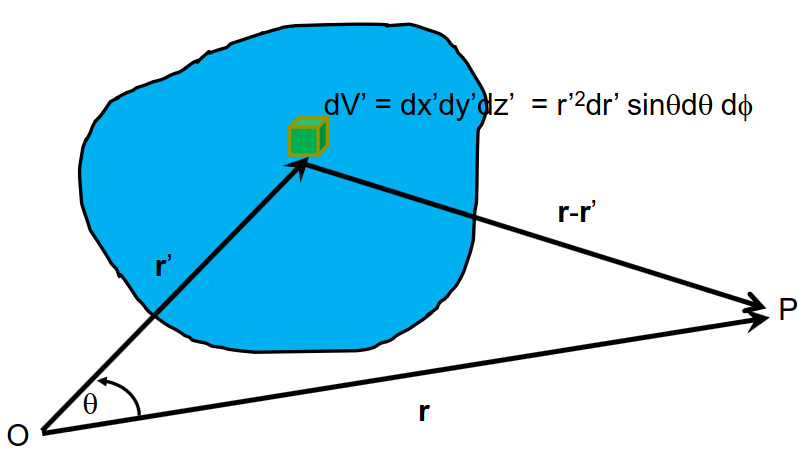
\includegraphics[width=200pt]{1.png}
    \caption{}
    \label{fig:pot}
\end{figure}
Let us analyse $|\vb{r} - \vb{r}'|$ more closely. We can find that,
\begin{equation}
\begin{split}
    |\vb{r} - \vb{r}'|^2 & = r^2 + (r')^2 - 2\vb{r}\cdot\vb{r}' \\
    & = r^2 + (r')^2 -2rr'\cos\theta,
\end{split}
\end{equation}
which is the cosine rule for a triangle between O, $\vb{r}$, and $\vb{r}'$, as in figure \ref{fig:pot}. This is important as it allows us to integrate the potential over a volume using polar coordinates. And thus, to find the total potential at a point $\vb{r}$, we integrate \eqref{potint} over a volume,
\begin{equation}
    \Phi(\vb{r}) = -G_N \int_V \frac{\rho(\vb{r}')}{|\vb{r} - \vb{r}'|}\dd{V}'.
\end{equation}
\textbf{NOTE:} $\Phi$ satisfies the Poisson equation, $\nabla^2\Phi = 4\pi G_N \rho$, where $\nabla^2 = \grad \cdot \grad$.
\subsection{Important Integral}
We will soon prove Newton's shell theorem, but we must first compute an important integral,
\begin{equation}
    I(a,b) = \int_0^{\pi} \frac{\sin\theta}{(a^2 + b^2 - 2ab\cos\theta)^{1/2}}\dd{\theta}.
\end{equation}
This results in,
\begin{equation}
    I(a,b) = \frac{1}{ab} = \left\{\left[(a+b)^2\right]^{\frac{1}{2}}-\left[(a\mp b)^2\right]^{\frac{1}{2}}\right\}
\end{equation}
which can be simplified as,
\begin{equation}
    I(a,b) = \begin{cases}
        \frac{2}{a} & a > b  \\
        \frac{2}{b} & b < a
    \end{cases}
\end{equation}
\subsection{Newton's Shell Theorem}
Let us consider a spherically symmetric shell of mass $M$ and radius $R$. We know,
\begin{align}
    \sigma & = \frac{M}{4\pi R^2} & \dd{A}' = R^2\sin{\theta}\dd{\theta}\dd{\phi}.
\end{align}
So, the potential is given by,
\begin{equation}
    \begin{split}
        \Phi(\vb{r}) & = -\frac{G_NM}{4\pi R^2}\int_0^{2\pi}\dd{\phi} \int_0^{\pi}\frac{R^2\sin\theta}{(r^2 + R^2 - 2rR\cos\theta)^{\frac{1}{2}}}\dd{\theta} \\
        & = -\frac{G_NM}{2}I(r,R).
    \end{split}
\end{equation}
We must now consider the cases where our point is \textbf{outside} the shell ($r > R$) and \textbf{inside} the shell ($r < R$),
\begin{equation}
    \Phi(\vb{r}) = \begin{dcases}
        -\dfrac{G_NM}{r} & r > R \\
        -\dfrac{G_NM}{R} & r < R
    \end{dcases}
\end{equation}
We can see that for $r < R$, the gravitational potential is constant. This implies that inside the shell there is no net force, as they all balance out due to the spherical symmetry of the shell. 
\subsection{Spherically symmetric mass distribution}
We will now calculate the potential of a spherically symmetric mass distribution, with density,
\begin{equation}
    \rho(\vb{r}) =
    \begin{cases}
        \rho(r) & r < R \\
        0 & r > R
    \end{cases}
\end{equation}
We can integrate over an infinitesimal potential, 
\begin{equation}
    \dd{\Phi(\vb{r})} = -G_N \frac{\rho(\vb{r}')}{(r^2 + (r')^2 - 2rr'\cos\theta)^{\frac{1}{2}}}\dd{V}',
\end{equation}
for each case. \\\\
For $r > R$,
\begin{equation}
    \begin{split}
        \Phi(\vb{r}) & = -G_N \int_0^R\rho(r')(r')^2\dd{r'}\int_0^{2\pi}\dd{\phi}\int_0^{\pi}\frac{\sin\theta}{(r^2+(r')^2 - 2rr'\cos\theta)^{\frac{1}{2}}}\dd{\theta} \\
        & = -2\pi G_N\int_0^R\rho(r')(r')^2\dd{r'}I(r,r').\\
        r > R \implies r' < r \implies & = -\frac{4\pi G_N}{r}\int_0^R\rho(r')(r')^2\dd{r'} = \frac{G_NM_{\text{tot}}}{r}
    \end{split}
\end{equation}
which is consistent with the potential due to a point particle.\\\\
Now considering the case $r < R$, we will be required to split the integral, such that we have one limit $0 \to r$ and then $r \to R$. Thus we obtain an integral,
\begin{equation}
    \Phi(\vb{r}) = -4\pi G_N \left\{ \frac{1}{r} \int_0^r \rho(r')(r')^2\dd{r'} + \int_r^R\rho(r')r'\dd{r'} \right\}.
\end{equation}
Let us take the derivative with respect $r$ in order to get an expression for the force within the mass and to get better intuition into what is happening in this setup,
\begin{equation}
\begin{split}
    \dv{\Phi(\vb{r})}{r} & = -4\pi G_N \left\{-\frac{1}{r^2}\int_0^r\rho(r')(r')^2\dd{r'}\right\} \\
    & = \frac{G_NM(r)}{r^2},
\end{split}
\end{equation}
where $M(r)$ is the mass inside the radius $r$. Thus, the force inside the mass is,
\begin{equation}
    \frac{1}{m}\vb{F} = -\dv{\Phi}{r}\vu{r} = - \frac{G_NM(r)}{r^2}\vu{r}
\end{equation}
as expected.

\section{Motion in a central potential}
In this section, we will be deriving the equations of motion required in order to be able to work in a centre-of-mass frame of 2 bodies under a \textbf{central force} This is useful as we know that the centre-of-mass frame is inertial. We can further simplify problems by always setting $\Dot{R} = 0$. Further, the equation of motion we can derive turns the the 3 dimensional problem into a 1 dimensional one, only dependent of $r$.
\\\\
We will then define a specific general potential such that, $U \propto \frac{1}{r}$, analogous to electrostatics and Newtonian gravity, by which we will be able to prove Kepler's laws:
\begin{klaw}
    Planetary orbits around the sun are elliptical with the sun at one of 2 foci.
\end{klaw}
\begin{klaw}
    Lines between the planet and the sun sweep out equal areas in equal intervals.
\end{klaw}
\begin{klaw}
    The orbital period of a planet squared is proportional to the cube of the semi-major axis.
\end{klaw}
\subsection{Energy in a Central Potential}
Let us recall that the force in the COM frame is,
\begin{equation} \label{reducedforce}
    \mu \Ddot{\vb{r}} = \vb{F} = -\dv{U}{r}\vu{r}.
\end{equation}
We understand that $\vb{r}\cdot\vb{r} = r^2 \implies A\vb{r}\cdot\Dot{\vb{r}} = Ar\Dot{r}$, thus, $\vu{r}\cdot\Dot{\vb{r}} = \Dot{r}$. Then, taking the dot product of \eqref{reducedforce} and $\Dot{r}$ yields,
\begin{equation}
    \mu \Dot{\vb{r}}\cdot \Ddot{\vb{r}} = -\Dot{r}\dv{U}{r} = -\dv{U}{t},
\end{equation}
\textbf{NOTE:} $\Dot{\vb{r}} \cdot \Ddot{\vb{r}} = \frac{1}{2}\dv{}{t}\left[\Dot{\vb{r}}^2\right]$, thus we can integrate,
\begin{equation}
    -U = \frac{1}{2}\mu\int\dv{}{t}\left[\Dot{\vb{r}}^2\right]\dd{t} = \frac{1}{2}\Dot{\vb{r}}^2 + E.
\end{equation}
where $E$ is the constant of integration. We can then rearrange to get the expression,
\begin{equation}
    E = \frac{1}{2}\mu\Dot{r}^2 + U(\vb{r}),
\end{equation}
implying that the energy of the system is constant.
\subsection{Angular Momentum}
We know the angular momentum in a COM frame is given by,
\begin{equation}
    \vb{L} = \mu\vb{r} \cross \Dot{\vb{r}}.
\end{equation}
Calculating the torque shows,
\begin{equation}
    \dv{\vb{L}}{t} = \mu(\Dot{\vb{r}}\cross\Dot{\vb{r}} + \vb{r}\cross\Ddot{\vb{r}}) = \vb{0}
\end{equation}
thus the angular momentum is constant, and thus is conserved in a COM frame. \\\\
Further, computing the dot product of angular momentum with $\Dot{\vb{r}}$ yields,
\begin{equation}
    \vb{L}\cdot\Dot{\vb{r}} = \mu\vb{r}\cross\Dot{\vb{r}} = 0,
\end{equation}
thus the angular momentum is perpendicular to velocity, implying the motion is in a plane. \\\\
We can use plane polar co-ordinates to describe the motion. This allows us to rewrite,
\begin{align}
    E &= \frac{1}{2}\mu(\Dot{r}^2 + r^2\Dot{\theta}^2) + U(r), & \vb{L} & = \mu\vb{r}\cross(\Dot{r}\vb{e}_{r} + r\Dot{\theta}\vb{e}_{\theta}) = \mu r^2 \Dot{\theta} \vb{e}_z,
\end{align}
and conclude the magnitude of $\vb{L}$ is a constant,
\begin{equation}
    L = \mu r^2 \Dot{\theta}.
\end{equation}
Thus, we can rewrite the total energy of our system as,
\begin{equation}
    E = \frac{1}{2}\mu \Dot{r}^2 + \frac{L^2}{2\mu r^2} + U(\vb{r}) = \frac{1}{2}\mu \Dot{r}^2 + U_{\text{eff}}(\vb{r}) \label{equationofmotioncentral}
\end{equation}
where,
\begin{equation}
    U_{\text{eff}}(r) = \frac{L^2}{2\mu r^2} + U(\vb{r}).\label{effectivepotential}
\end{equation}
Thus, \eqref{equationofmotioncentral} is the general equation of motion of a system under a central potential.
\subsubsection{Kepler's Second Law}
\begin{figure}[h]
    \centering
    \begin{tikzpicture}
        \node[isosceles triangle, draw, fill=red!30, isosceles triangle apex angle=30,rotate=270, minimum size = 3cm, draw=none](T)  at(0,0) {};   
        \node at (T.apex) {\textbullet};
        \draw[->] (T.apex) -- (T.left corner);
        \draw[->] (T.apex) -- (T.right corner);
        \node at (T.center) {$\dd{A}$};
        \node[anchor=east] at (T.right corner) {$\vb{r}$};
        \node[anchor=west] at (T.left corner) {$\vb{r} + \dd{\vb{r}}$};
        \node[anchor=south] at (0,-4) {$\dd{\theta}$};
    \end{tikzpicture}
    \caption{}
    \label{fig:tri}
\end{figure}
We are able to prove this by the conservation of angular momentum we have derived. Let us consider an infinitesimal area $\dd{A}$ (figure \ref{fig:tri}). The area under this element is,
\begin{equation}
    \dd{A} = \frac{1}{2}r^2\dd{\theta}.
\end{equation}
The change in time is then,
\begin{equation}\label{K2}
    \dv{A}{t} = \frac{1}{2}\Dot{r}^2 \Dot{\theta} = \frac{L}{2\mu}
\end{equation}
which is constant, thus proving Kepler's second law as a consequence of the conservation of angular momentum. As we have not made any assumptions about the potential, we can also say that Kepler's second law is true for all systems under a central force.
\subsection{Trajectory of a COM system under a specific potential}
We will attempt to find an expression for $r(\theta)$, or the trajectory of the system. We will want to find an equation of motion which is easily solved. Firstly, let us define,
\begin{equation}
    \frac{1}{r} = u
\end{equation}
where,
\begin{align}
    \Dot{u} &= - \frac{\Dot{r}}{r^2} = -\Dot{r}u^2, & \Dot{\theta} &= \frac{Lu^2}{\mu}
\end{align}
follows. We can then derive an equation of motion,
\begin{equation}
    \left(\dv{u}{\theta}\right)^2 = \left(\frac{\Dot{u}}{\Dot{\theta}}\right)^2 = \left(\frac{\mu}{L}\right)^2\Dot{r}^2 = \frac{2\mu}{L^2}\left[E - U\left(\frac{1}{u}\right)\right] - u^2,
\end{equation}
where we can define a specific general potential,
\begin{equation}
    U(r) = -\frac{\alpha}{r},
\end{equation}
where $\alpha$ is analogous to $G_Nm_1m_2$ for newtonian gravity or $\frac{q_1q_2}{4\pi\epsilon_0}$. Thus, 
\begin{equation}
    \left(\dv{u}{\theta}\right)^2 = \frac{2\mu}{L^2}(E + \alpha u) - u^2.
\end{equation}
We can then define,
\begin{align}
    r_0 &= \frac{L^2}{\alpha \mu} & u_0 &= \frac{1}{r_0}  & \varepsilon^2 = 1 + \frac{2L^2E}{\alpha^2 \mu}, \label{propertiespotential}
\end{align}
so we can further reduce the equation of motion,
\begin{equation}
    \left(\dv{u}{\theta}\right)^2 = \varepsilon^2u_0^2 - (u-u_0)^2.
\end{equation}
Finally, we define
\begin{equation}
    \overline{u} = \frac{u-u_0}{\varepsilon u_0},
\end{equation}
to arrive at a trivial differential equation,
\begin{equation}
    \dv{\overline{u}}{\theta} = \sqrt{1 - \overline{u}^2}.
\end{equation}
Before we integrate, we must choose an appropriate substitution for $\overline{u}$. We understand, 
\begin{itemize}
    \item $\dv{u}{\theta} \propto -\Dot{r}$.
    \item It is convenient to choose a condition such that $\overline{u} = 0$ at $\theta = \frac{\pi}{2}$ as that is when the trajectory crosses the axis.
\end{itemize}
Thus, $\overline{u} = \cos\theta$. This yields the solution,
\begin{equation}
    r(\theta) = \frac{r_0}{1 + \varepsilon\cos\theta}. \label{potgravitysolutio}
\end{equation}
\textbf{NOTE:} This is only a solution for a potential in the form $U \propto -\frac{1}{r}$. \\\\
Converting \eqref{potgravitysolutio} into Cartesian co-ordinates, we find,
\begin{equation}
    r + \varepsilon x = r_0
\end{equation}
and,
\begin{equation}
\begin{split}
    x^2 + y^2 = r_0^2 -2\varepsilon r_0 x + \varepsilon^2x^2 \\
    \implies (1 - \varepsilon^2)x^2 + y^2 + 2\varepsilon r_0x = r_0^2, \label{quadmotion}
\end{split}
\end{equation}
which for $0 \leq \varepsilon < 1$, rearranges to,
\begin{equation}
    \frac{\left(x + \frac{\varepsilon r_0}{1-\varepsilon}\right)^2}{\left(\frac{r_0}{1-\varepsilon^2}\right)^2} + \frac{y^2}{\left(\frac{r_0}{\sqrt{1-\epsilon^2}}\right)^2}  = 1.
\end{equation}
Now, defining,
\begin{align}
    a & = \frac{r_0}{1-\varepsilon^2}, & b & = \frac{r_0}{\sqrt{1-\varepsilon^2}}, & X &= x + \frac{\varepsilon r_0}{1-\varepsilon}, & Y &= y
\end{align}
we obtain,
\begin{equation}
    \frac{X^2}{a^2} + \frac{Y^2}{b^2} = 1
\end{equation}
which is the equation for an ellipse, thus proving Kepler's first law. We can then ascribe physical meaning to some constants which we have defined,
\begin{align}
    a && \implies && \text{Semi major axis} \\
    b && \implies && \text{Semi minor axis} \\
    \varepsilon && \implies && \text{Eccentricity of orbit} \\
    r_0 && \implies && \text{Radius when orbit is a circle/}
\end{align}
We can obtain further identities,
\begin{align}
    b &= a \sqrt{1 - \varepsilon^2} & \varepsilon^2 = 1 - \left(\frac{b}{a}\right)^2
\end{align}
We note that,
\begin{equation}
    1 - \varepsilon^2 = -2\frac{Er_0}{\alpha},    
\end{equation}
implying that $E < 0$. Given the limits we imposed on $\varepsilon$, we can also state that the energy of the system must be in the limits,
\begin{equation}
    -\frac{\alpha}{2r_0} \leq E < 0,
\end{equation}
\subsubsection{Kepler's Third Law}
If we integrate the expression of Kepler's second law with time, \eqref{K2}, we can obtain an expression for the period,
\begin{equation}
    \frac{LT}{2\mu} = A = \pi ab = \pi a^2 \sqrt{1-\varepsilon^2}.
\end{equation}
We can then derive, given that $r_0 = \frac{L^2}{\alpha \mu}$, that,
\begin{equation}
    \frac{L}{\mu} = \left(\frac{\alpha}{\mu}\right)^{\frac{1}{2}}r_0^{\frac{1}{2}} = \left(\frac{\alpha}{\mu}\right)^{\frac{1}{2}}a^{\frac{1}{2}}\sqrt{1-\varepsilon^2}
\end{equation}
Thus,
\begin{equation}
    T = 2\pi \frac{\mu}{L} a^2 \sqrt{1 - \varepsilon^2} = 2\pi a^{\frac{3}{2}}\left(\frac{\mu}{\alpha}\right)^{\frac{1}{2}}
\end{equation}
We can rewrite this,
\begin{equation}
    T^2 = \frac{4\pi^2 \mu}{\alpha}a^3 \implies \text{ Kepler's Third Law}
\end{equation}
\section{Motion in Effective Potential}
We previously solved an equation of motion using an expression of potential for a specific form of potential. The total energy is in the form, \eqref{equationofmotioncentral} and the effective potential is \eqref{effectivepotential}. We will think about this equation of motion more analytically by analysing the potential curve, and identifying stationary points.
\subsection{$\alpha > 0$}
\begin{figure}
    \centering
    \begin{tikzpicture}
        
        \begin{axis}[
            axis lines=center,
            ylabel = $U_{\text{eff}}$,
            xlabel = $r$,
            y label style ={anchor=east},
            domain=0:12,
            restrict y to domain=-4:4,
            ymax=2,
            ymin=-3,
            xmax=12,
            xmin=-1,
            ticks=none]
            \addplot[samples=200,color=red,very thick] {((-4)*(x^-1)) + ((4^2)/(2*4*x^2))};
            \addplot +[mark=none,dashed,color=black,thick] coordinates {(1, -4) (1, 3)};
            \addplot +[mark=none,dashed,color=black,thick] coordinates{(-1,-2) (13,-2)};
            \node at (axis cs:8,-1.6) {$\dfrac{-\mu\alpha^2}{2L^2} = -\dfrac{\alpha}{2r_0} = \dfrac{U(r_0)}{2}$};
            \node at (axis cs:2.5,1.6) {$r_0 = \dfrac{L^2}{\mu\alpha}$};
        \end{axis}
    \end{tikzpicture}
    \caption{Graph of effective potential for $\alpha > 0$.}
    \label{fig:alphamorethan}
\end{figure}
Let us take the derivative of effective potential,
\begin{equation}
    \dv{U_\text{eff}(r)}{r} = -\frac{L^2}{\mu r^3} + \frac{\alpha}{r^2}.
\end{equation}
We can then deduce there will be a stationary point is,
\begin{equation}
    \frac{L^2}{\alpha \mu} = r_0.
\end{equation}
We can then take the second derivative,
\begin{equation}
    \dv[2]{U_\text{eff}(r)}{r} = \frac{1}{r^4}\left(\frac{3L^2}{\mu} - 2\alpha r\right)
\end{equation}
which we can evaluate for $r = r_0$ as,
\begin{equation}
    \dv[2]{U_\text{eff}(r)}{r} = \frac{L^2}{\mu r_0^4} > 0.
\end{equation}
We can then conclude that this is a minimum stationary point. We can then plot the effective potential with $r$ to obtain a graph (see figure \ref{fig:alphamorethan}). We can then analyse this for different energies. 
\subsubsection{1. $E = -\frac{\mu\alpha^2}{2L^2}$, $\varepsilon=0$}
The particle is at minimum potential. Thus,
\begin{itemize}
    \item $\implies$ Stable circular orbit at $r = r_0$.
    \item $\implies$ There may be small oscillations in the orbit with an equivalent spring constant of,
    \begin{equation}
        k = \frac{L^2}{\mu r_0^4}.
    \end{equation}
\end{itemize}
\subsubsection{2. -$\frac{\mu\alpha^2}{2L^2} < E < 0$, $0 < \varepsilon < 1$}
This will result in the particle rolling around the bottom of the potential, but not having enough energy to escape the orbit completely or fall into the centre.
\\\\
For energies $E \geq 0$, and $\varepsilon \geq 1$, particles follow hyperbolic motion, which is discussed in a later section.
\subsection{$\alpha < 0$}
\begin{figure}
    \centering
     \begin{tikzpicture}
        \begin{axis}[
            axis lines=center,
            ylabel = $U_{\text{eff}}$,
            xlabel = $r$,
            y label style ={anchor=east},
            x label style = {anchor=west},
            domain=0:25,
            restrict y to domain=0:5,
            ymax=2,
            ymin=0,
            xmax=20,
            xmin=-1,
            ticks=none]
            \addplot[samples=200,color=red,very thick] {((4)*(x^-1)) + ((4^2)/(2*4*x^2))};
        \end{axis}
    \end{tikzpicture}
    \caption{Graph of effective potential for $\alpha < 0$.}
    \label{fig:negativealpbha}
\end{figure}
This does not occur in Newtonian gravity, but can occur in electrostatics. There are no stationary points, thus all energies result in hyperbolic motion and there is no stability. The particle will simply hit the potential barrier, then bounce back. I.E., motion is always a hyperbola.
\subsection{Stability in Circular Orbits}
If we consider the Taylor expansion about $r_0$ of the stationary orbit, we will get an equation of simple harmonic motion, where,
\begin{equation}
    k = \dv[2]{U_\text{eff}}{r}(r_0).
\end{equation}
If $\dv[2]{U_{\text{eff}}}{r}(r_0) > 0$, our orbit is stable, but unstable is $\dv[2]{U_{\text{eff}}}{r}(r_0) < 0$. \\\\
\textbf{Stable orbits} are able to trap particles in potential wells, leading to oscillatory/orbital motion. 

\noindent
\textbf{Unstable orbits} are such that if a particle's orbit deviates from $r = r_0$, it's motion will change dramatically. A particle with $E < U_{\text{eff}}(r_0)$ will come from infinity, but will be unable to break past the potential barrier. A particle which comes from $r < r_0$ will simple fall into $r = 0$ (the centre of the orbit). A particle which has energy $E > U_{\text{eff}}(r_0)$ will also simply fall into the centre. Figure \ref{fig:unstable} shows an example of a case where $U(r) = -\frac{\alpha}{r^5}$.
\begin{figure}
    \centering
    \begin{tikzpicture}
        
        \begin{axis}[
            axis lines=center,
            ylabel = $U_{\text{eff}}$,
            xlabel = $r$,
            y label style ={anchor=east},
            x label style = {anchor=west},
            domain=-0.5:7,
            restrict y to domain=-4:1.8,
            ymax=1.7,
            ymin=-0.2,
            xmax=6,
            xmin=-1,
            ticks=none]
            \addplot[samples=200,color=red,very thick] {((-0.5)*(x^-5))+ ((0.8^2)/(0.5*x^2))};
            \addplot +[mark=none,dashed,color=black, thick] coordinates {(0.9921, -1) (0.9921, 1.8)};
            \addplot +[mark=none,dashed,color=black,thick] coordinates{(-0.5,0.7802) (7,0.7802)};
            \node at (axis cs:3,0.9) {$U_{\text{eff}}(r_0)$};
            \node at (axis cs:2.3,1.5) {$r_0 = \left(\dfrac{5\mu\alpha}{L^2}\right)^{\frac{1}{3}}$};
        \end{axis}
    \end{tikzpicture}
    \caption{Graph of unstable, effective potential for $\alpha > 0$.}
    \label{fig:unstable}
\end{figure}
\section{Conic Sections}
We are now going to consider solutions for motion where $\varepsilon \geq 1$
\subsection{$\varepsilon = 0$}
In this case, the motion is a parabola in the form,
\begin{equation}
    y^2 = r_0^2 - 2r_0x.
\end{equation}
\subsection{$\varepsilon > 0$}
In this case, we can complete the square on the expression \eqref{quadmotion},
\begin{equation}
    \left(x + \frac{\varepsilon r_0}{1-\varepsilon^2}\right)^2 + \frac{y^2}{1-\varepsilon^2} = \frac{r_0^2}{\left(1-\varepsilon^2\right)^2}.
\end{equation}
In this case, the coefficient of $y^2$ is negative, so we must make the transformation,
\begin{equation}
    (X,Y) = \left(x- \frac{\varepsilon r_0}{\varepsilon^2 -1},y\right) = (x - \sqrt{a^2 + b^2}),y),
\end{equation}
where we define,
\begin{align}
    a & = \frac{r_0}{\varepsilon^2 - 1} & b & = \frac{r_0}{\sqrt{\varepsilon^2 - 1}} & \varepsilon & = 1 + \left(\frac{b}{a}\right)^2.
\end{align}
We then get a curve,
\begin{equation}
    \frac{X^2}{a^2} - \frac{Y^2}{b^2} = 1
\end{equation}
which is in the general form of a hyperbola, with asymptotes,
\begin{equation}
    Y = \pm \left(\frac{b}{a}\right)
\end{equation}
\subsection{Generating conic sections}
All of the possible curves under a central potential have the form of a conic section. We are able to generate these through the use of a \textbf{directrix}.
\begin{figure}[h]
    \centering
    \begin{tikzpicture}
        \coordinate (O) at (0,0);
        \coordinate (F) at (2,0);
        \coordinate (P) at (1,1.5);
        \coordinate (D) at (4,1.5);
        \node[anchor=north east] at (O) {$O$};
        \draw[axis] (O) -- (0,3) node[anchor = east] {$Y$};
        \draw[axis] (O) -- (5,0) node[anchor=north] {$X$};
        \node[anchor=north] at (F) {$F(f,0)$};
        \draw[thick] (F) -- (P) node[midway,anchor=east] {$\varepsilon|PD|$};
        \node at (P) {\textbullet};
        \node[anchor=south] at (P) {$P(X,Y)$}; 
        \draw[dashed,thick] (4,-0.5) -- (4,3.5) node[anchor=west]{$X = d$};
        \draw[thick] (P) -- (D) node[midway,above] {$|PD|$};
        \node[anchor=west] at (D) {$D(d,Y)$};
        \draw[dashed] (F) -- (D);
    \end{tikzpicture}
    \caption{General directrix}
    \label{fig:directrix}
\end{figure}\\
We can first define a focus point, $F(f,0)$, and the directrix $D$ to be the vertical line generated by the locuses of points $(d,Y)$. We then demand $|PF| = \varepsilon|PD|$, which implies,
\begin{equation}
    \begin{split}
        (X-f)^2 + Y^2 = \varepsilon^2(X-d)^2 \\
        \implies (1-\varepsilon^2)X^2 + Y^2 - 2(f-\varepsilon^2d^2)X = \varepsilon^2d^2 - f^2.
    \end{split}
\end{equation}
which is in the same form as \eqref{quadmotion}. \\\\
Then, by choosing various values for the focal point and directrix, we can generate different conic sections. The choices we must make in order to generate various conic sections are shown in table \ref{tab:conicsectiontable}. We should also elaborate on a new variable presented called the \textbf{semi-latus rectum} $\ell$, which is the value of $Y$ when $X = f$. For elipses and hyperbolae, this is given by, $\ell = r_0$.
\begin{table}[h]
    \centering
    \begin{tabular}{C C C C}\toprule
         &  \text{\textbf{Ellipse}} &\text{\textbf{Hyperbola}} & \text{\textbf{Parabola}}\\
         \midrule
        f & (a^2-b^2)^{\frac{1}{2}} & (a^2 + b^2)^{\frac{1}{2}} & a \\ \midrule
        \ell & \dfrac{b^2}{a} & \dfrac{b^2}{a} & 2a \\\midrule
        \varepsilon & \left[1-\left(\dfrac{b}{a}\right)^2\right]^{\frac{1}{2}} & \left[1+\left(\dfrac{b}{a}\right)^2\right]^{\frac{1}{2}} & 1 \\ \midrule
        d & \pm \dfrac{a}{\varepsilon} & \pm \dfrac{a}{\varepsilon} & -a \\
        \bottomrule\end{tabular}
    \caption{Table of choices to generate conic sections.}
    \label{tab:conicsectiontable}
\end{table}

\chapter{Rigid Body Motion}
\section{Properties of a Rigid Body}
\begin{definition}[Rigid Body]
    A system of particle's in which the distance between them does not change regardless of the forces acting, such that their coordinates are,
    \begin{equation}
        \vb{r}^{(k)} = r_i^{(k)}\vb{e}_i
    \end{equation}
    such that,
    \begin{equation}
        r_{ij} = \left|\vb{r}^{(i)} - \vb{r}^{(j)}\right|
    \end{equation}
    is constant.
\end{definition}
\noindent
We only need 3 particles/reference points in order to describe a 3 dimensional rigid body. These points must not be in a straight line. These are the constraints of the body, and they will have 6 degrees of freedom corresponding to 3 translations and 3 rotations.\\\\
We can further define the following properties of a rigid body composed of a discrete number of particles, $N$. We can convert the discrete forms into continuous ones by using the \textit{continuum limit}, taking $\dd{M} = \rho \dd{V}$.
\begin{align}
    M & = \begin{dcases}
        \sum_{k=1}^Nm_k & \text{Discrete}\\
        \int\rho \dd{M} & \text{Continuous}
    \end{dcases} &&\implies&& \text{Total Mass}\label{eq:mass}\\
    \vb{R} & = \begin{dcases}
        \frac{1}{M}\sum_{k=1}^Nm_k\vb{r}^{(k)} & \text{Discrete} \\
        \frac{1}{M}\int \rho \vb{r}\dd{V} & \text{Continuous}
    \end{dcases} &&\implies&& \text{Position of centre of mass} \label{eq:com}\\
    \vb{P}^{\text{tot}} & = \begin{dcases}
        \sum_{k=1}^Nm_k \Dot{\vb{r}}^{(k)} & \text{Discrete} \\
        \int \rho\Dot{\vb{r}}\dd{V} & \text{Continuous}
    \end{dcases} &&\implies&& \text{Total linear momentum} \label{eq:linmom}\\
    \vb{L}^{\text{tot}} &= \begin{dcases}
        \sum_{k=1}^Nm_K\vb{r}^{(k)}\cross\Dot{\vb{r}}^{(k)} & \text{Discrete}\\
        \int \rho\left( \vb{r} \cross \Dot{\vb{r}}\right)\dd{V}& \text{Continuous}
    \end{dcases} &&\implies&& \text{Total angular momentum}\label{eq:angmom}\\
    T^{\text{tot}} &= \begin{dcases}
        \frac{1}{2}\sum_{k=1}^Nm_k\left|\Dot{\vb{r}}^{(k)}\right|^2 & \text{Discrete}\\
        \frac{1}{2}\int \rho |\Dot{\vb{r}}|^2\dd{V} & \text{Continuous}
    \end{dcases} &&\implies&& \text{Total kinetic energy} \label{eq:kin}
\end{align}
\section{Moment of Inertia Tensor}
Let us recall,
\begin{align}
    (\vb{A}\cross\vb{B})\cross\vb{C} & = (\vb{A}\cdot \vb{C})\vb{B} - (\vb{B}\cdot \vb{C})\vb{A} \\
    \vb{C}\cross(\vb{A}\cross\vb{B}) & = (\vb{B}\cdot\vb{C})\vb{A} - (\vb{A}\cdot \vb{C})\vb{B} \\
    (\vb{A}\cross\vb{B})\cdot(\vb{C}\cross\vb{D}) &= (\vb{A}\cdot\vb{C})(\vb{B}\cdot\vb{D}) - (\vb{A}\cdot\vb{D})(\vb{B}\cdot\vb{C})
\end{align}
and,
\begin{equation}
    \Dot{\vb{r}}^{(k)}|_S = \Dot{\vb{r}}^{(k)}|_{S'} + \vb*{\omega}\cross\vb{r}^{(k)}. \label{angorsom}
\end{equation}
We can then define $S'$ to be the frame where $\Dot{\vb{r}}^{(k)}|_{S'} = 0$. Substituting \eqref{angorsom} into \eqref{eq:angmom} then gives,
\begin{equation}
    \vb{L}^{(tot)} = \sum_{k=1}^Nm_k\vb{r}^{(k)}\cross\left(\vb*{\omega}\cross\vb{r}^{(k)}\right) = \sum_{k=1}^Nm_K\left[\left|\vb{r}^{(k)}\right|^2\vb*{\omega} - \left(\vb{r}^{(k)}\cdot\vb*{\omega}\right)\vb{r}^{(k)}\right],
\end{equation}
then rewriting this in index notation,
\begin{equation}
    \begin{split}
        L_i^{(\text{tot})} & = \sum_{k=1}^Nm_k\left[\left|\vb{r}^{(k)}\right|^2\omega_i - r_j^{(k)}\omega_jr_i^{(k)}\right] \\
        & = I_{ij}\omega_j
    \end{split}
\end{equation}
where $I_{ij}$ is the moment of inertia tensor \textit{about the origin}, 
\begin{equation}
    I_{ij} = \begin{dcases}
        \sum_{k=1}^Nm_k\left[\left|\vb{r}^{(k)}\right|^2\delta_{ij} - r_i^{(k)}r_j^{(k)}\right] & \text{Discrete} \\
        \int \rho\left(r^2\delta_{ij} - r_ir_j\right)\dd{V} & \text{Continuous}
    \end{dcases}
\end{equation}
\textbf{NOTE:} When talking about the moment of inertia it, must always be \textit{about a point} with \textit{respect to some axis}.
\\\\Let us now write $\vb{r}^{(k)} = \vb{R} +\vb{r}'^{(k)}$, where $\vb{r}'^{(k)}$ is the position of the $k$th particle with respect to the centre of mass, which must satisfy,
\begin{equation}
    \sum_{k=1}^N  m_k\vb{r}'^{(k)} \equiv 0. \label{masssum}
\end{equation}
Let us now substitute these into expressions for \eqref{eq:linmom} and \eqref{eq:angmom}. Superscript "$\text{com}$" indicates the centre of mass and "$\text{rot}$" indicates the rotating frame.
\begin{equation}
\begin{split}
    \vb{P}^{\text{tot}} & = \sum_{k=1}^Nm_k\left(\Dot{\vb{R}} + \vb*{\omega}\cross\vb{r}'^{(k)}\right) = \left(\sum_{k=1}^Nm_k\right)\Dot{\vb{R}} + \vb*{\omega}\cross\left(\sum_{k=1}^Nm_k\vb{r}'^{(k)}\right) \\ 
    & = M\Dot{\vb{R}} \equiv \vb{P}^{\text{com}}
\end{split}
\end{equation}
\begin{equation}
\begin{split}
    \vb{L}^{\text{tot}} & = \sum_{k=1}^Nm_k \left(\vb{R}+\vb{r}'^{(k)}\right) \cross\left(\Dot{\vb{R}}+\vb*{\omega}\cross\vb{r}'^{(k)}\right) \\
    & = \sum_{k=1}^Nm_k \left[\vb{R}\cross\Dot{\vb{R}} + \vb{r}'^{(k)}\cross\Dot{\vb{R}} + \vb{R}\cross\left(\vb*{\omega}\cross\vb{r}'^{(k)}\right) + \vb{r}'^{(k)}\cross\left(\vb*{\omega}\cross\vb{r}'^{(k)}\right)\right] \\
    & = \vb{R}\cross M \Dot{\vb{R}} + \sum_{k=1}^N\left[m_K\vb{r}'^{(k)}\cross\left(\vb*{\omega}\cross\vb{r}'^{(k)}\right)\right] \\
    &= \vb{L^{\text{com}}} + \vb{L^{\text{rot}}}
\end{split}
\end{equation}
We define,
\begin{align}
    L_i^{\text{com}} & = M\epsilon_{ijk}R_j\Dot{R}_k = \epsilon_{ijk}R_kP_k^{\text{com}} \\
    L_i^{\text{rot}} & = I'_{ij}\omega_j
\end{align}
where $I'_{ij}$ is the moment of inertia about the centre of mass, given by,
\begin{equation}
    I'_{ij} = \sum_{k=1}^Nm_k\left[\left|\vb{r}'^{(k)}\right|^2\delta_{ij} - r_i'^{(k)}r_j'^{(k)}\right] \neq I_{ij}.
\end{equation}
We can also express the total kinetic energy as,
\begin{equation}
\begin{split}
    T^{\text{tot}} & = \frac{1}{2}\sum_{k=1}^Nm_k\left|\Dot{\vb{R}} + \vb*{\omega}\cross\vb{r}'^{(k)}\right|^2 \\
    & =  \frac{1}{2}\sum_{k=1}^Nm_k\left[\left|\Dot{\vb{R}}\right|^2 + \Dot{\vb{R}}\cdot\vb*{\omega}\cross\vb{r}'^{(k)} + \left|\vb*{\omega}\cross\vb{r}'^{(k)}\right|^2\right] \\
    & = \frac{1}{2}M\Dot{\vb{R}}^2 + \frac{1}{2}\sum_{k=1}^Nm_k\left|\vb*{\omega}\cross\vb{r}'^{(k)}\right|^2 \\
    & = T^{\text{com}} + T^{\text{rot}}
\end{split}
\end{equation}
where we define,
\begin{align}
    T^{\text{com}} & = \frac{1}{2}M\left|\Dot{\vb{R}}\right|^2 \\
    T^{\text{rot}} & = \frac{1}{2}\sum_{k=1}^Nm_k\left\{\left|\vb*{\omega}^2\right|\left|\vb{r}'^{(k)}\right|^2-\left|\vb{r}'^{(k)}\cdot\vb*{\omega}\right|^2\right\} = \frac{1}{2}\omega_iI_{ij}\omega_j.
\end{align}
\subsubsection{Calculating the moment of inertia tensor}
The moment of inertia integral can be given in matrix form,
\begin{equation}
    \mathbf{I} = \int \dd{M}\begin{pmatrix}
        y^2 + z^2 & -xy & -xz \\
        -yx & z^2 + x^2 & -yz \\
        -zx & -zy & x^2 + y^2
    \end{pmatrix}
\end{equation}
\section{Parallel axis theorem - Steiner's Theorem}
Let us consider a collection of particles whose position vector $\vb{r}^{(k)}$, which can be written as,
\begin{equation}
    \vb{r}^{(k)} = \vb{R} + \vb{r}'^{(k)}.
\end{equation}
We can then deduce,
\begin{align}
    \left|\vb{r}^{(k)}\right|^2 & =  \left|\vb{R}\right|^2 + 2\vb{R}\cdot\vb{r}'^{(k)} + \left|\vb{r}'^{(k)}\right| \\
    r_i^{(k)}r_j^{(k)} & = R_iR_j + R_ir'^{(k)}_j + R_ir'^{(k)}_i + r'^{(k)}_ir'^{(k)}_j.
\end{align}
Let us recall \eqref{masssum}. This then implies,
\begin{equation}
    I_{ij} = M\left(\left|\vb{R}\right|^2\delta_{ij}-R_iR_j\right) + I_{ij}', \label{parallelaxis}
\end{equation}
where, in this final formula given by \eqref{parallelaxis}, $\vb{R}$ is the position about which $I_{ij}$ is, and $I_{ij}'$ is the moment of inertia about the centre of mass.
\subsubsection{Perpendicular Axis Theorem}
We will consider a lamina such that,

\begin{align}
    \dd{M} = \sigma(x,y) && r_i = \left\{x,y,0\right\}.
\end{align}
then,
\begin{equation}
    I_{ij} = \int\int\sigma(x,y)\dd{x}\dd{y}\begin{pmatrix}
        y^2 & -xy & 0 \\
        -xy & x^2 & 0 \\
        0 & 0 & x^2 + y^2
    \end{pmatrix}.
\end{equation}
It is then clear,
\begin{equation}
    I_{11} + I_{22} = I_{33}.
\end{equation}

\section{The Principles Axis}
We can relate the angular momentum between two frames $S$ and $S'$ by a rotation matrix $O_{ij}$,
\begin{equation}
    L_i' = O_{ij}L_j
\end{equation}
such that $O_{ij}$ satisfies,
\begin{equation}
    O_{ik}O_{jk} = \delta_{ij}.
\end{equation}
If the angular momentum is in the form $L_i = I_{ij}\omega_j$ in all frames of reference, then,
\begin{equation}
    L_i' = I_{ij}'\omega_j' \implies O_{ij}L_j = O_{ij}I_{jk}\omega_k = I_{ij}'O_{jk}\omega_k
\end{equation}
where $I_{ij}'$ is the moment of inertia in $S'$.
\\\\
This must be true for all $\omega_k$, such that,
\begin{equation}
    \begin{split}
        &O_{ij}I_{jk} = I_{ij}'O_{jk} \implies O_{lk}O_{ij}I_{jk} = I_{ij}'O_{jk}O_{lk} = I_{ij}'\delta_{jl} = I_{il}'\\
        \implies&I_{il}' = O_{ij}O_{lk}I_{jk} \implies \text{2 rotation matrices $\therefore$ I is a rank 2 tensor}
    \end{split}
\end{equation}
\subsection{Diagonalization of symmetric matrices}
\begin{theorem}
    Any real, symmetric, square matrix $A$ is diagonizable, such that there exists a matrix $P$ where,
    \begin{equation}
        P^{-1}AP = D = \text{diag}\left(d^{(1)},d^{(2)},\ldots,d^{(3)}\right)
    \end{equation}
    where $n$ is the dimension of the matrix.
\end{theorem}
In order to construct $P$ and $D$ we must find the \textit{Eigenvalues} and \textit{Eigenvectors} of $A$. Let us recall, to setup an Eigenvalue problem by considering,
\begin{equation}
    A\vb{E}^{(k)} = \lambda^{(k)}\vb{E}^{(k)}
\end{equation}
and finding the non-trivial solutions when the determinant is 0, such that,
\begin{equation}
    \det{A - \lambda\mathbb{1}_n} = 0
\end{equation}
where $\lambda^{(k)}$ are the Eigenvalues, $\vb{E}^{(k)}$ are the Eigenvectors, and $\mathbb{1}_n$ is an identity matrix of dimension $n$.
\\\\
Solving then yields,
\begin{align}
    P=(\vb{E}^{(1)},\vb{E}^{(2)},\ldots,\vb{E}^{(n)}) && D = \text{diag}(\lambda^{(1)},\lambda^{(2)},\ldots,\lambda^{(n)})
\end{align}
We able to choose our Eigenvectos to be orthonormal, such that,
\begin{equation}
    \vb{E}^{(k)}\cdot\vb{E}^{(m)} = \delta_{km}
\end{equation}
which leads to \textit{orthogonal diagonalisation}, by whereby,
\begin{equation}
    \begin{split}
        &P^{-1}=P^T; PP^T=\mathbb{1}_n \\
        \implies&\text{$P$ is orthogonal}.
    \end{split}
\end{equation}
Further, orthogonal diagonalisation implies that,
\begin{equation}
    A = PDP^T = \sum_{k=1}^n \lambda^{(k)}\vb{E}^{(k)}(\vb{E}^{(k)})^T,
\end{equation}
and thus, for any vector $\vb{x}$, 
\begin{equation}
    \vb{x}^{T}A\vb{x} = \sum_{k=1}^n\lambda^{(k)}\left((\vb{E}^{(k)})^T\vb{x}\right)^2 \label{vectordiagonlisation}
\end{equation}
\subsection{Diagonalization of the moment of inertia tensor}
The moment of inertia tensor is symmetric, and can thus be diagonalized. We can then write a diagonalized moment of inertia tensor,
\begin{equation}
    \Hat{I}_{ij} = \begin{pmatrix}
        I^{(1)} & 0 & 0 \\
        0 & I^{(2)} & 0 \\
        0 & 0 & I^{(3)}
    \end{pmatrix}
\end{equation}
where $I^{(n)}$ are the Eigenvalues of the moment of inertia tensor. The moment of inertia tensor will then be given by,
\begin{equation}
    I = P\Hat{I}P^T.
\end{equation}
What we have essentially done by diagonalizing the moment of inertia tensor is rotated our frame of reference so we use the Eigenvectors of $I$ as the basis vectors. We are then working in the \textbf{principle axis} of the rigid body. If we call this new frame $S'$, we can rewrite the angular momentum as,
\begin{equation}
    \vb{L}' = \Hat{I}\vb*{\omega}'
\end{equation}
where,
\begin{align}
    \vb{L}' = P^T\vb{L} && \vb*{\omega}' = P^T\vb*{\omega} = \begin{pmatrix}
        \left(\vb{E}^{(1)}\right)^T\vb*{\omega} \\ \left(\vb{E}^{(2)}\right)^T\vb*{\omega} \\ \left(\vb{E}^{(3)}\right)^T\vb*{\omega}
    \end{pmatrix}.
\end{align}
By \eqref{vectordiagonlisation}, we obtain an expression for kinetic energy in terms of the Eigenvalues and Eigenvectors of the moment of inertia tensor,
\begin{equation}
    T = \frac{1}{2}\sum_{k=1}^3I^{(k)}\left[\left(\vb{E}^{(k)}\right)^T\vb*{\omega}\right]^2.
\end{equation}
\section{Euler's Equation}
We are able to relate the rate of change of angular momentum to torque, $\vb{M}$. Defining $S$ as a static inertia frame and $S'$ as the fixed body, rotating frame, we have,
\begin{equation}
\begin{split}
    \vb{M}& = \Dot{\vb{L}}|_S = \Dot{\vb{L}}|_{S'} + \vb*{\omega}\cross\vb{L}
    \\ & = I\Dot{\vb*{\omega}} + \vb*{\omega}\cross\left(I\vb*{\omega}\right)
\end{split}
\end{equation}
which is known as Euler's equation. Since we can always diagonalise the moment of inertia, we can rewrite the angular momentum as,
\begin{equation}
    \vb{L} = I \vb*{\omega} = \begin{pmatrix}
        I^{(1)}\omega_1 \\ I^{(2)}\omega_2\\ I^{(3)}\omega_3
    \end{pmatrix}
\end{equation}
and 
\begin{equation}
    I\Dot{\vb*{\omega}} = \begin{pmatrix}
        I^{(1)}\Dot{\omega_1} \\ I^{(2)}\Dot{\omega_2} \\ I^{(3)}\Dot{\omega_3}
    \end{pmatrix}.
\end{equation}
Thus, we can rewrite Euler's equations as,
\begin{equation}
    \begin{split}
        M_1 & = I^{(1)}\Dot{\omega_1} + (I^{(3)} - I^{(2)})\omega_2\omega_3  \\
        M_2 & = I^{(2)}\Dot{\omega_2} + (I^{(1)} - I^{(3)})\omega_3\omega_1 \\
        M_3& = I^{(2)}\Dot{\omega_2} + (I^{(2)} - I^{(1)})\omega_1\omega_2
    \end{split}
\end{equation}
\newpage
\section{Free Rotation of a Symmetric Top}
\begin{figure}
	\centering
	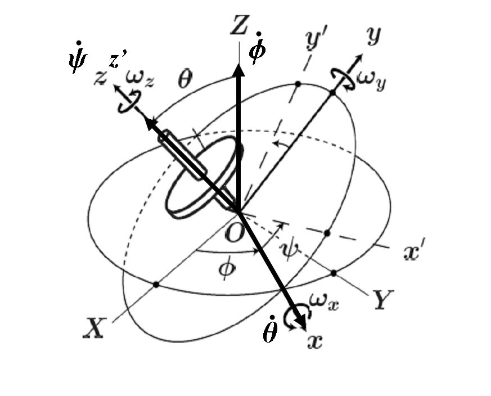
\includegraphics[width=300pt]{spinningtop.png}
	\caption{A diagram showing a spinning top as well as all of the Euler angles. $\psi$ is the spin, $\phi$ is the precession, and $\theta$ is the nutation.}
	\label{top}
\end{figure}
Free rotation occurs when $\Dot{\vb*{\omega}} = \vb{M} = 0$. For the case when $\vb*{\omega}$ is parallel to $\vb{L}$, $\vb*{\omega}$ is an Eigenvector of the moment of inertia tensor.
\\\\
Let us assume that the rigid body is symmetric about the axis such that $I_{11} = I_{22} = I$. We will not assume time-independent motion about the 2 other axis. Euler's equations for free rotation cause us to have to accept that, $\Dot{\omega}_3 \equiv 0$, thus we can set
\begin{equation}
    \omega_3 = \omega_t
\end{equation}
constant, such that $\omega_t$ is the angular velocity of the top. We can then define,
\begin{align}
    \Dot{\omega}_1 = -\Omega\omega_2 && \Dot{\omega}_2 = \Omega\omega_1
\end{align}
where
\begin{equation}
    \Omega = \left(\frac{I^{(3)}-I}{I}\right)\omega_t.
\end{equation}
By taking another time derivative, we obtain the differential equation,
\begin{equation}
    \Ddot{\omega}_1 = -\Omega^2\omega_1
\end{equation}
whose solutions are,
\begin{align}
    \omega_1 = A\cos{(\Omega t + \phi)} && \omega_2 = A\sin{(\Omega t + \phi)}.
\end{align}
Thus, the angular velocity in the principle axis frame is given by,
\begin{equation}
    \vb*{\omega} = \begin{pmatrix}
        \omega_1 \\ \omega_2 \\ \omega_3
    \end{pmatrix} = \left(A\cos(\Omega t + \phi)\right)\vb{E}^{(1)} + \left(A\sin(\Omega t + \phi)\right)\vb{E}^{(2)} + \omega_t\vb{E}^{(3)}.
\end{equation}
Further, we have shown that $\omega_1^2 + \omega_2^2 = A^2$ is a constant of motion.
\\\\
We are now interested how the spinning top behaves in the lab frame.  Let us consider the angular moment and rotational kinetic energy,
\begin{align}
	L_i = I_{ij}\omega_j && T_R = \frac{1}{2}\omega_i I_{ij}\omega_j = \frac{1}{2} \omega_iL_i = \frac{1}{2}\vb*{\omega}\cdot\vb{L}.
\end{align}
Since $T_R$ is constant, so must $\vb*{\omega}\cdot\vb{L}$. We can then explicitly show,
\begin{align}
	|\vb*{\omega}| = \sqrt{A^2 + \omega_t^2} && |\vb{L}|=\sqrt{I^2A^2 + \left(I^{(3)}\right)^2 \omega_t^2} && \vb*{\omega}\cdot\vb{L}=IA^2 + I^{(3)} \omega_t^2
\end{align}
are all constant.\\\\
By Newton's second law, $\vb{L}$ must be constant, and we will choose it to be in the $\vb{e}_3$ direction, such that,
\begin{equation}
	\vb{L} = L\vb{e}_3.
\end{equation}
Thus, $\vb*{\omega}$ will rorate about $\vb{L}$, maintaining a constant angle between the two. HOwever, $\vb{L}$ is not constant in the body-fixed frame.
\\\\
Let us attempt to visualise the evolution of $\vb{E}_3$ in the lab frame. First,
\begin{equation}
	\vb{L} - I\vb*{\omega} = (I^{(3)} - I)\omega_t\vb{E}_3
\end{equation}
which indicates that $\vb{L}$, $\vb*{\omega}$, and $\vb{E}_3$ lie in a plane. We can write,
\begin{equation}
	\vb*{\omega} = \frac{L}{I}\vb{e}_3 - \left(\frac{I^{(3)} 0 I}{I}\right)\omega_t \vb{E}_3.
\end{equation}
Let us now define $\Theta$ as the angle fixed between $\vb{E}_3$ and $\vb{L}$, and $\Phi \equiv \Phi(t)$ to be the angle of rotation about the third axis. We can write,
\begin{equation}
	\vb{E}_3 = \cos\Theta\vb{e}_3 + \sin\Theta(\cos\phi\vb{e}_1 + \sin\phi\vb{e}_2)
\end{equation}
and
\begin{equation}
	\Dot{\vb{E}}_3 = \Dot{\Phi}\sin\Theta(-\sin\Phi\vb{e}_1 + \cos\Phi\vb{e}_2) \label{4.65}
\end{equation}
thus, $\Dot{\vb{E}}_3 = \vb*{\omega}\cross\vb{E}_3$, and,
\begin{equation}
	\Dot{\vb{E}}_3 = \frac{L}{I}\vb{e})3 \cross\vb{E}_3 = \frac{L}{I}\sin\Theta(\cos\Phi \vb{e}_2 - \sin\Phi \vb{e}_1) \label{4.66}.
\end{equation}
Combining \eqref{4.65} and \eqref{4.66}, we see that $\Dot{\Phi} = \frac{L}{I}$ when $\Theta \neq 0$.
\\\\
\textbf{ASIDE:} The case where $\Theta = 0$ corresponds to fixed roation about hte principle axis $\vb{E}_3$.
\\\\
We can deduce,
\begin{equation}
	\vb{L}\cdot\vb{E}_3 = L \cos\Theta = I^{(3)}\omega_t.
\end{equation}
From which we can deduce $\vb*{\omega}$ can $\vb{E}_3$ precess about $\vb{L}$ in the lab frame with constant frequency,
\begin{equation}
	\Omega_p = \Dot{\Phi} = \frac{L}{I} = \frac{I^{(3)}\omega_t}{I\cos\Theta}.
\end{equation}
To clarify, the top spins with frequency $\omega_t$ about the symmetric axis, which is in turn precesses around $\vb{L}$ with frequency $\Omega_p$. THe body will appear to "wobble". The body will have two ways of wobbling. We can attempt to visualise this by considering a "space cone", whose axis is fixed, and a "body cone" which moves with the body and rolls around on the space cone.
\\\\
The body may exhibit \textit{prolate} roation if $I^{(3)} < I$, so the body cone rolls on the outside of the space cone. 
\\\\
THe body may also exhbiit \textit{oblate} procession when $I^{(3)}>I$ and the body cone rolls about the inside of the space cone.
\subsection{Intermediate Axis Theorem}
Let us consider a spinning top with no symmetry, defined by a constant angular velocity $\omega_t$ but with small perturbations in all directions, such that,
\begin{equation}
	\vb*{\omega} = \begin{pmatrix}
		\delta \omega_1 & \delta \omega_2 & \omega_t + \delta\omega_3
	\end{pmatrix}.
\end{equation}
Subsituting this into Euler's equations implies that $\delta \Dot{\omega}_3 = 0$, so,
\begin{align}
	I_1\delta\Dot{\omega}_1 &= (I_2 - I_3)\omega_t\delta\omega_2 \\
	I_1\delta\Dot{\omega}_2 = (I_3 - I_1)\omega_t\delta\omega_1\end{align}
If we differentiate $\delta \omega_1$ and substitute for $\delta\Dot{\omega}_2$, we deduce,
\begin{equation}
	\delta \Ddot{\omega}_1 + \Omega^2\delta\omega_1 = 0
\end{equation}
where
\begin{equation}
	\Omega^2 = \frac{(I_3 - I_2)(I_3-I_1)}{I_1I_2}\omega_t^2
\end{equation}
and similarly for $\omega_2$. From this, we can determine that there is only stable motion when the rate of change of angular velocity opposes angular velocity, i.e.,
\begin{align}
	I_3 > I_1 && \text{AND} && I_3 > I_2
\end{align}
OR
\begin{align}
	I_3 < I_1 && \text{AND} && I_3 < I_2
\end{align}
and is unstable for,
\begin{align}
	I_2 > I_3 > I_1 && \text{or} && I_1 > I_3 > I_2.
\end{align}
This is the intermediate axis theorem. 
\section{Gyroscopes}
A gyroscope can be thought of as a heavy spinning top, such that gravity and other external forces act. These forces are:
\begin{itemize}
	\item \textbf{Gravity}, $\vb{F}_g = m\vb{g}$, whcih acts throughout the centre of mass at $\vb{r} = R\vb{e}_r$. 
	\item \textbf{Contact force}, the point of contact will be assumed to be fixed and will impart no torque.
\end{itemize}
The torque due to gravity is then,
\begin{equation}
	\vb{M} = \vb{r} \times m\vb{g} = mg R \sin\theta \vb{e}_{\phi}. \label{torque due to gravity}
\end{equation}
The polar angles are used to describe the orientation of the principal axis which in turn point in the direction of $\vb{e}_r$. These angles are $\psi$,$\theta$, and $\phi$, as in figure \ref{top}, and are known as Euler angles. Since the torque only acts in $\vb{e}_{\phi}$, angular momentum will be conserved in other directions. The top is further symmetric, such that the moments of inertia are, 
\begin{align}
	I_1 = I_2 = I && \text{and} && I_3.
\end{align}
If we recall \eqref{derivativeofbasis}, since the top spins with angular velocity $\Dot{\psi}$,
\begin{equation}
	\vb*{\omega} = (\Dot{\phi}\cos\theta + \Dot{\psi})\vb{e}_r -\Dot{\phi}\sin\theta\vb{e}_{\theta} + \Dot{\theta}\vb{e}_{\phi},
\end{equation} 
thus we can write the angular momentum,
\begin{equation}
	\vb{L} = I_3(\Dot{\phi}\cos\theta + \Dot{\psi})\vb{e}_r + I(\Dot{\theta}\vb{e}_{\phi} - \Dot{\phi}\sin\theta\vb{e}_{\theta}).
\end{equation}
Newton's second law gives us $\Dot{\vb{L}} = \vb{M}$, thus, 
\begin{equation}
	\frac{1}{2}\dv{}{t}|\vb{L}|^2 = \vb{M}\cdot\vb{L}.
\end{equation}
If $\theta$ is constant, $\vb{M}\cdot\vb{L}=0$ and $|\vb{L}|$ is constant. We can then compute,
\begin{equation}
	\begin{split}
		\Dot{\vb{L}} & = I_3(\Ddot{\phi}\cos\theta - \Dot{\phi}\Dot{\theta}\sin\theta + \Ddot{\psi})\vb{e}_r \\
		& + \left[I_3(\Dot{\phi}\cos\theta + \Dot{\psi})\Dot{\phi}\sin\theta + I(\Ddot{\theta} - \Dot{\phi}^2\sin\theta\cos\theta)\right]\vb{e}_{\phi} \\
		& + \left[I_3(\Dot{\phi}\cos\theta + \Dot{\psi})\Dot{\theta} - I(\Ddot{\theta}\sin\theta + 2\Dot{\phi}\Dot{\theta}\cos\theta)\right]\vb{e}_{\theta}.
	\end{split}
\end{equation}
Now by applying Newton's second law and using \eqref{torque due to gravity}, we get,
\begin{align}
	\Ddot{\phi}\cos\theta - \Dot{\phi}\Dot{\theta}\sin\theta + \Ddot{\psi} & = 0 \label{expression1} \\
	I_3(\Dot{\phi}\cos\theta + \Dot{\psi})\Dot{\phi}\sin\theta + I(\Ddot{\theta} - \Dot{\phi}^2\sin\theta\cos\theta) & = 0 \label{expression2} \\
	I_3(\Dot{\phi}\cos\theta + \Dot{\psi})\Dot{\theta} - I(\Ddot{\theta}\sin\theta + 2\Dot{\phi}\Dot{\theta}\cos\theta) & = mgR\sin\theta \label{expression3}
\end{align}
From \eqref{expression1},
\begin{equation}
	\dv{}{t}(\Dot{\phi} + \Dot{\psi}) = 0
\end{equation}
which implies that the angular velocity vector along the spin axis of the top is,
\begin{equation}
	\omega_2 = \Dot{\phi}\cos\theta + \Dot{\psi},
\end{equation}
and is constant.
\\\\
Similarly, for \eqref{expression2},
\begin{equation}
	I_3\omega_3\Dot{\theta} - \frac{I}{\sin\theta}\dv{}{t}(\Dot{\phi}\sin^2\theta) = 0
\end{equation}
implying,
\begin{equation}
	I_3\omega_3 \cos\theta + I\Dot{\phi}\sin^2\theta \equiv bI
\end{equation}
is constant. Rearranging this,
\begin{equation}
	\Dot{\phi} = \frac{bI - I_3 \omega_3 \cos\theta}{I\sin^2\theta} = \frac{b-a\cos\theta}{\sin^2\theta}
\end{equation}
for,
\begin{equation}
	a = \frac{I_3\omega_3}{I}.
\end{equation}
Let us now define,,
\begin{align}
	L = Ia && K = Ib. 
\end{align}
We can rewrite \eqref{expression3} as,
\begin{equation}
	\Ddot{\theta} = \sin\theta\left(\frac{1}{2}\beta - a \Dot{\phi} + \Dot{\phi}^2\cos\theta\right)
\end{equation}
where
\begin{equation}
	\beta = \frac{2mgR}{I}.
\end{equation}
Let us consider a case where $\theta = \theta_0$ is constant and $\Dot{\psi} = \omega_s$, $\Dot{\phi}=\Omega_p$ is constnat, where,
\begin{equation}
	\Omega_s = \frac{I}{I_3}a - \Omega_p\cos\theta_0
\end{equation}
and $\Omega_p$ is a solution to,
\begin{equation}
	\cos\theta \Omega_p^2 - a\Omega_p + \frac{1}{2}\beta = 0
\end{equation}
where 
\begin{equation}
	\Omega_p = \frac{a}{2\cos\theta_0}\left[1\pm\left(1 - \frac{2\beta\cos\theta_0}{a^2}\right)^{\frac{1}{2}}\right]
\end{equation}
when
\begin{equation}
	\cos\theta_0 < \frac{a^2}{2\beta} = \frac{I_3^2\omega_3^2}{4mgRI}.
\end{equation}
If $a^2 > 2\beta$, then there is always such a solution. If $a^2 < 2\beta$, there exists a critical angle,
\begin{equation}
	\theta_{\text{crit}} = \cos^{-1}\left(\frac{a^2}{2\beta}\right)\text{ where } \theta_0 > \theta_{\text{crit}},
\end{equation}
i.e., there is no solution when $\theta_0 = 0$. This is a condition where,
\begin{equation}
	\omega_3 > \frac{\sqrt{2mgRI\cos\theta_0}}{I_3}\label{condition}
\end{equation}
which is necessary to prevent the top from falling down.
\\\\
We can investigate the motion further by analysing solutions in the limit,
\begin{equation}
	\frac{2\beta \cos\theta_0}{a^2} << 1
\end{equation}
which is the equivalent to ignoring gravity. This results in the positive root,
\begin{equation}
	\Omega_p^{\text{fast}} - \frac{a}{\cos\theta_0} = \frac{I_3\omega_3}{I\cos\theta_0} = \frac{L}{I\cos\theta_0}.
\end{equation}
and the negative root,
\begin{equation}
	\Omega_p^{\text{slow}}=\frac{\beta}{2a} = \frac{mgR}{I_3\omega_3} = \frac{mgR}{L}.
\end{equation}
The slow solution is seen in free rotation.
\\\\
We can further analyse the energy in the system. Th erotational kinetic energy satisfies $\Dot{T}_R = \vb*{\omega}\cdot\vb{M}$. Computing this in our case,
\begin{equation}
	\vb*{\omega}\cdot{\vb{M}} = mgR\Dot{\theta}\sin\theta = -mgR\dv{}{\theta}\cos\theta
\end{equation}
from which we can deduce,
\begin{equation}
	E = T_R + V = T_R + mgR\cos\theta
\end{equation}
is constnat. We can rewrite this as,
\begin{equation}
	E = \frac{1}{2}I_3(\Dot{\phi}\cos\theta + \Dot{\psi})^2 + \frac{1}{2}I(\Dot{\theta}^2 + \Dot{\phi}^2 \sin^"\theta)+ mgR\cos\theta.
\end{equation}
Let us now define,
\begin{equation}
	\bar{E}= \frac{E - \frac{1}{2}I_3\omega_3^2}{I} = \frac{1}{2}\Dot{\theta} + \frac{1}{2}\left(\frac{b-a\cos\theta}{\sin\theta}\right)^2
 + \frac{mgR}{I}\cos\theta
 \end{equation}
so, we can define  an effective potential such that $\bar{E} = \frac{1}{2}\Dot{\theta}^2 + U_{\text{eff}}(\theta)$,
\begin{equation}
	U_{\text{eff}} = \frac{1}{2}\left[\left(\frac{b-a\cos\theta}{\sin\theta}\right)^2 \beta\cos\theta \right].
\end{equation}
We have thus found a way to describe the effective motion of the gyroscope in 1 dimension. An example of a plot of this potential is show in figure \ref{effpotgyro}.
\begin{figure}
	\centering
	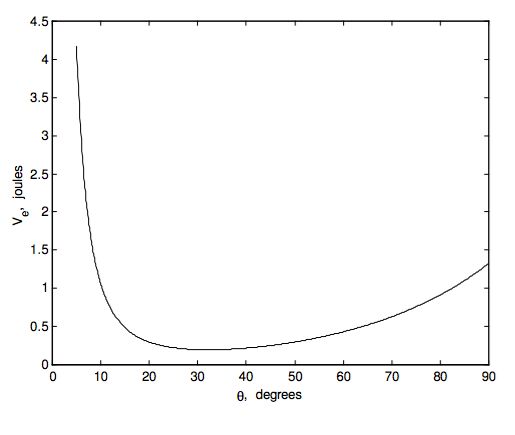
\includegraphics[width=200pt]{FigureIV.32.png}
	\caption{A plot of the effective potential of a gyroscope.}
	\label{effpotgyro}
\end{figure}
\\\\
A basic analysis is laid out below:
\begin{itemize}
	\item The initial state of the system is governed by conserved quantities.
	\item The motion of $\theta$ takes place between $\theta_1 < \theta < \theta_2$ which can be computed by setting $\Dot{\theta} = 0$.
	\begin{itemize}
		\item The particle will \textit{nutate} between $\theta_1$ and $\theta_2$. This nutation can occur in different nutation modes, which depend on sign sof $\Omega_p$ and initial conditions.
		\item Figure \ref{unidirectional} shows unidirectional precession.
		\item Figure \ref{looping} shows looping precession.
		\item Figure \ref{cuspidal} shows cuspidal precession.
	\end{itemize}
	\item Uniform precession occurs when $\Dot{\theta} = \Ddot{\theta} = 0$ at $\theta = \theta_0$, which occurs at $\bar{E} = U_{\text{eff}}$, $\Dot{U}_{\text{eff}} = 0$.
	\item We can impose $\theta = 0$ as a solution, so long as \eqref{condition} is met.
\end{itemize}
\begin{figure}
	\centering
	\begin{subfigure}[b]{0.3\textwidth}
		\centering
		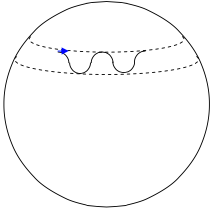
\includegraphics[width=130pt]{nutation1.png}
		\caption{This is unidirectional precession}
		\label{unidirectional}
	\end{subfigure}
	\begin{subfigure}[b]{0.3\textwidth}
		\centering
		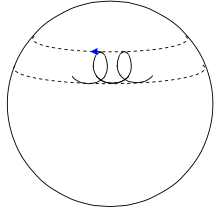
\includegraphics[width=130pt]{nutation3.png}
		\caption{This is looop precession.}
		\label{looping}
	\end{subfigure}
	\begin{subfigure}[b]{0.3\textwidth}
		\centering
		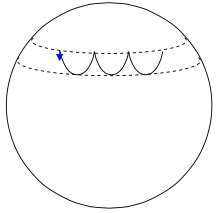
\includegraphics[width=130pt]{nutation4.png}
		\caption{This is cuspidial precession.}
		\label{cuspidal}
	\end{subfigure}
	\caption{Figures showing different nutation modes.}
\end{figure}
\chapter{Special Relativity}

\appendix
\chapter{Examples}
\section{$r_{\text{min}}$ and $r_{\text{max}}$}
We get turning points in $r$ when $\Dot{r} = 0$. Thus, by \eqref{equationofmotioncentral} and by defining $u = \frac{1}{r}$, we are able to obtain the quadratic,
\begin{equation}
    \frac{L^2}{2\mu}u^2 + U(r) - E = 0.
\end{equation}
For a central potential in the form, $U(r) = -\frac{\alpha}{r} = -\alpha u$, we obtain solutions,
\begin{equation}
    u = \frac{\alpha \pm \sqrt{\alpha^2 + \frac{2EL^2}{\mu}}}{\frac{L^2}{\mu}}.
\end{equation}
Let us now recall \eqref{propertiespotential}, 
\begin{align}
    u_0 = \frac{\alpha \mu}{L^2} && \varepsilon^2 = 1 + \frac{2L^2E}{\alpha \mu},
\end{align}
we can then conclude,
\begin{align}
    r_\text{min} = r(1-\varepsilon) && r_{\text{max}} = r(1+\varepsilon).
\end{align}
\section{Matrix Decomposition}
\begin{theorem}
    Any matrix $\mathcal{M}$ can be written as the sum of its symmetric, $\mathcal{S}$, and anti-symmetric, $\mathcal{T}$, components such that,
    \begin{equation}
        \mathcal{M} = \mathcal{S} + \mathcal{T}.
    \end{equation}
\end{theorem}
\begin{proof}
    Consider,
    \begin{equation}
        \begin{split}
            &(\mathcal{M} + \mathcal{M}^T)_{ij} = \mathcal{M}_{ij} + \mathcal{M}_{ij}^T = \mathcal{M}_{ji}^T + \mathcal{M}_{ji} = (\mathcal{M}^T + \mathcal{M})_{ji} = (\mathcal{M} + \mathcal{M}^T)_{ji} \\
            \implies&(\mathcal{M} + \mathcal{M}^T)\text{ is symmetric}\implies \mathcal{S} = 2(\mathcal{M} + \mathcal{M}^T).
        \end{split}
    \end{equation}
    Then, consider,
    \begin{equation}
    \begin{split}
            &(\mathcal{M} - \mathcal{M}^T)_{ij} = \mathcal{M}_{ij} - \mathcal{M}_{ij}^T = \mathcal{M}_{ji}^T - \mathcal{M}_{ji} = (\mathcal{M}^T - \mathcal{M})_{ji} = -(\mathcal{M} - \mathcal{M}^T)_{ji} \\
            \implies&(\mathcal{M} - \mathcal{M}^T)\text{ is anti-symmetric}\implies \mathcal{T} = 2(\mathcal{M} - \mathcal{M}^T).
        \end{split}
    \end{equation}
    Now,
    \begin{equation}
        \begin{split}
            \mathcal{M} = \frac{1}{2}\mathcal{M} + \frac{1}{2}\mathcal{M} + \frac{1}{2}\mathcal{M}^T - \frac{1}{2}\mathcal{M}^T & = \frac{1}{2}(\mathcal{M} + \mathcal{M}^T) + \frac{1}{2}(\mathcal{M} -\mathcal{M}^T) \\
            & = \mathcal{S} + \mathcal{T}
        \end{split}
    \end{equation}
\end{proof}
\chapter{Moments of Inertia}
\section{Solid Cylinder}
We will consider a solid cylinder about its centre of mass of radius $R$ and a height $h$. Let us define,
\begin{align}
    \dd{M} & = \rho\dd{V} = \rho r \dd{r}\dd{\theta}\dd{z} & \rho & = \frac{M}{\pi R h}.
\end{align}
We use coordinates,
\begin{align}
    x = r \cos\theta && y = r\sin\theta.
\end{align}
Then,
\begin{equation}
\begin{split}
    \mathbf{I} & = \rho\int_0^Rr\dd{r}\int_0^{2\pi}\dd{\theta} \int_{-\frac{1}{2}h}^{\frac{1}{2}h}\begin{pmatrix}
        r^2\sin^2\theta & -r^2\cos\theta\sin\theta & rz\cos\theta \\
        -r^2\sin\theta\cos\theta & z^2 + r^2\cos^2\theta & -rz\sin\theta \\
        -rz\cos\theta & -rz\sin\theta & r^2
    \end{pmatrix}\dd{z}
    \\
    & = M\begin{pmatrix}
        \frac{1}{4}R^2 + \frac{1}{12}h^2 & 0 & 0\\
        0 & \frac{1}{4}R^2 + \frac{1}{12}h^2 & 0 \\
        0 & 0 & \frac{1}{2}R^2 \\
    \end{pmatrix}
\end{split}
\end{equation}
\section{Cylindrical Shell}
Similarly to \textbf{A.1},
\begin{align}
    \dd{M} & = \sigma \dd{A} = \sigma R \dd{\theta}\dd{z} & \sigma & = \frac{M}{2\pi R h}. 
\end{align}
Then,
\begin{equation}
\begin{split}
    \mathbf{I} & = \rho\int_0^Rr\dd{r}\int_0^{2\pi}\dd{\theta} \int_{-\frac{1}{2}h}^{\frac{1}{2}h}\begin{pmatrix}
        r^2\sin^2\theta & -r^2\cos\theta\sin\theta & rz\cos\theta \\
        -r^2\sin\theta\cos\theta & z^2 + r^2\cos^2\theta & -rz\sin\theta \\
        -rz\cos\theta & -rz\sin\theta & r^2
    \end{pmatrix}\dd{z}
     \\
    & = M\begin{pmatrix}
        \frac{1}{2}R^2 + \frac{1}{12}h^2 & 0 & 0\\
        0 & \frac{1}{2}R^2 + \frac{1}{12}h^2 & 0 \\
        0 & 0 & R^2 \\
    \end{pmatrix}
\end{split}
\end{equation}
\section{Solid Sphere}
We will assume a uniform density. Then,
\begin{equation}
    I_{ij} = \frac{2}{5}MR^2\delta_{ij}.
\end{equation}
\section{Spherical Shell}
Once again assuming uniform density,
\begin{equation}
    I_{ij} = \frac{2}{3}MR^2\delta_{ij}.
\end{equation}
\section{Solid cone}
Assuming uniform density, the moment of inertia about the apex is,
\begin{equation}
    I_{ij} = \frac{3}{5}M\text{diag}\left(h^2+\frac{1}{4}R^2,h^2+\frac{1}{4}R^2,\frac{1}{2}R^2\right).
\end{equation}
\section{Ellipsoid}
A solid ellipsoid with semi-radii $(a,b,c)$ has a moment of inertia about its centre of mass,
\begin{equation}
    I_{ij} = \frac{1}{M}\text{diag}\left(b^2+c^2, c^2+a^2, a^2+b^2\right).
\end{equation}
\textbf{NOTE:} For an ellipsoid, we have,
\begin{equation}
	\dd{V} = abcr^2\sin\theta\dd{r}\dd{\theta}\dd{\phi}.
\end{equation}
\section{Thin Rod}
This method using the parallel axis theorem. Let us consider a rod of length $L$, then
\begin{align}
    \dd{M} = \mu\dd{\ell} && \mu = \frac{M}{L} && \vb{r} = (x,y,z) = \ell(0,1,0).
\end{align}
We can then deduce,
\begin{equation}
    \mathbf{I}' = \mu\int_{-\frac{1}{2}L}^{\frac{1}{2}L}\dd{\ell}\text{diag}(\ell^2,0,\ell^2) = \frac{1}{12}ML^2\text{diag}(1,0,1).
\end{equation}
We can then calculate the moment of inertia about one end of the ro. We have,
\begin{equation}
    \vb{R} = \frac{1}{2}L\begin{pmatrix}
        0 \\ 1 \\ 0
    \end{pmatrix}
\end{equation}
then,
\begin{equation}
    |\vb{R}|^2\delta_{ij} - R_iR_j = \frac{1}{4}L^2\text{diag}(1,0,1)
\end{equation}
so,
\begin{equation}
    \mathbf{I} = \frac{1}{12}ML^2\text{diag}(1,0,1) + \frac{1}{4}ML^2\text{diag}(1,0,1) = \frac{1}{3}ML^2\text{diag}(1,0,1).
\end{equation}
\chapter{Rotating Reference Frames on Earth}
\noindent We will be considering a non-inertial reference frame on the surface of the earth, with the $x$-axis pointing east, $y$-axis pointing north, and the $z$-axis pointing "up" or towards space. We will then define the following vectors (using Cartesian basis vectors), 
\begin{align}
    \vb*{\omega} &= \omega\begin{pmatrix}
        0 \\
        \cos\lambda \\
        \sin\lambda
    \end{pmatrix} 
    &
    \vb{g} &= \begin{pmatrix}
        0 \\
        0 \\
        -g
    \end{pmatrix}.
\end{align}

\section{Pendulum at rest}
\begin{figure}[h]
    \centering
    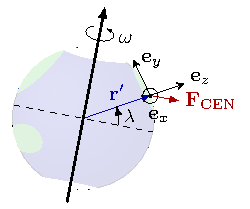
\includegraphics[width=250pt]{document_ACDF_10245.pdf}
    \caption{Visualisation of the centrifugal force.}
    \label{fig:CF}
\end{figure}
\noindent
The only inertial force acting on objects at rest in a rotating frame is the centrifugal force. This force has the effect of reducing the weight of an observer on earth. However,  this force will act radially outwards from the axis of rotation ($\vb{e}_r$) rather than in $\vb{e}_z$.  \\\\
We will now consider a pendulum at rest at some inclination on the earth, with a position vector,
\begin{equation}
    \vb{r}' = \begin{pmatrix}
        0 \\
        0 \\
        R_E
    \end{pmatrix}.
\end{equation} 
The centrifugal force will cause the pendulum to be slightly deflected by an angle $\alpha$ as the centrifugal force does not point in its weight.
\\\\
We understand that the centrifugal acceleration is,
\begin{equation}
    \frac{1}{m}\vb{F}_{\text{CEN}} = \vb*{\omega}\cross(\vb*{\omega}\cross\vb{r}')
\end{equation}
which we can rewrite using the identity,
\begin{equation}
    \vb{A}\cross(\vb{B}\cross\vb{C}) = (\vb{A}\cdot\vb{C})\vb{B} - (\vb{A}\cdot\vb{B})\vb{C},
\end{equation}
then,
\begin{equation}
    \frac{1}{m}\vb{F}_{\text{CEN}} = \omega^2\vb{r}' - (\vb*{\omega}\cdot\vb{r}')\vb*{\omega} = \omega^2R_E\begin{pmatrix}
        0 \\
        -\sin\lambda\cos\lambda \\
        \cos^2\lambda
    \end{pmatrix}.
\end{equation}
We can then consider the effective gravity felt by the observer in the non-inertial frame,
\begin{equation}
\begin{split}
    \vb{g}_{\text{EFF}} &= \vb{g} + \frac{1}{m}\vb{F}_{\text{CEN}}\\
    & = \vb{g} - \begin{pmatrix}
        0 \\
        -\omega^2R_E\sin\lambda\cos\lambda \\
        \omega^2R_E\cos^2\lambda
    \end{pmatrix} = \begin{pmatrix}
        0 \\
        \omega^2R_E\sin\lambda\cos\lambda \\
        -g + \omega^2R_E\cos^2\lambda
    \end{pmatrix}.
\end{split}
\end{equation}
We then obtain the magnitude and angle by usual means, approximating where appropriate,
\begin{equation}
\begin{split}
    |\vb{g}_{\text{EFF}}| &= g\left(1 - \frac{2\omega^2R_E}{g}\cos^2\lambda + \left(\frac{\omega^2R_E}{b}\right)^2\cos^2\lambda\right)^{\frac{1}{2}} \\
    & \approx g\left(1-\frac{\omega^2R_E}{g}\cos^2\lambda\right)
\end{split}
\end{equation}
\begin{equation}
\begin{split}
    \tan\alpha & = \frac{\omega^2R_E\sin\lambda\cos\lambda}{-g-\omega^R_E\cos^2\lambda} = \frac{\omega^2R_E}{g}\sin\lambda\cos\lambda\left(1-\frac{\omega^2R_E}{g}\cos^2\lambda\right)^{-1} \\
    \alpha & \approx \frac{R_E\omega^2}{g}\sin\lambda\cos\lambda
\end{split}
\end{equation}
\section{Particle falling to earth}
We will consider a particle falling to Earth from a height $h$ from rest under free fall, only considering its motion within the non-inertial frame. We will define the position vector of the object as,
\begin{equation}
    \vb{r}(t) = \begin{pmatrix}
        x(t) \\
        y(t) \\
        z(t)
    \end{pmatrix}
    \equiv 
    \begin{pmatrix}
        x\\
        y\\
        z
    \end{pmatrix} \equiv \vb{r}
\end{equation}
whose initial conditions are given by,
\begin{align}
    \vb{r}(0) & = \begin{pmatrix}
        0 \\
        0 \\
        R_E + h
    \end{pmatrix} 
    &
    \Dot{\vb{r}}(0) & = \vb{0}.
\end{align}
The equation of motion is given as follows,
\begin{equation}
    \Ddot{\vb{r}} = \vb{g} - 2\vb*{\omega}\times\Dot{\vb{r}} + \omega^2\vb{r} - (\vb{r}\cdot\vb*{\omega})\vb*{\omega}.
\end{equation}
The timescale of the rotation of the earth is much larger than the timescale of free fall under gravity. It is then useful to define a new timescale, along with an angular velocity unit vector
\begin{align}
    T& = \omega t & \vu*{\omega}=\frac{\vb*{\omega}}{\omega}.
\end{align}
This allows us to rewrite the equation of motion,
\begin{equation}
    \dv[2]{\vb{r}}{T} = \frac{\vb{g}}{\omega^2} - 2\vu*{\omega}\cross\dv{\vb{r}}{T} + \vb{r} - (\vb{r}\cdot\vu*{\omega})\vu*{\omega}.
\end{equation}
We can then write the equations of motion for each component,
\begin{align}\label{equations}
    \dv[2]{x}{T} &= x - 2\left(\dv{z}{t}\cos\lambda - \dv{y}{T}\sin\lambda\right) \\
    \dv[2]{y}{T} &= y - 2\dv{x}{T}\sin\lambda - \cos\lambda(y\cos\lambda + z\sin\lambda)\label{equations2} \\ 
    \dv[2]{z}{T} &= z - \frac{g}{\omega^2} - 2\dv{x}{T}\cos\lambda - \sin\lambda(y\cos\lambda + z\sin\lambda) \label{equations3}
\end{align}
It is very difficult to solve these equations generally, however a power series solution is valid as in most real-world scenarios, $$T << 1$$. First, we define,
\begin{equation}
\begin{split}
    \vb{r}(T) & = \vb{r}(0) + T\frac{\Dot{\vb{r}}(t)}{\omega} + \vb{A}T^2 + \vb{B}T^3 + \cdots \\
    & = \begin{pmatrix}
        0 \\ 0 \\ R_E + h
    \end{pmatrix} + \begin{pmatrix}
        A_1 \\ A_2 \\ A_3 
    \end{pmatrix}T^2 + \begin{pmatrix}
        B_1 \\ B_2 \\ B_3
    \end{pmatrix}T^3.
\end{split}
\end{equation}
The solutions are found by differentiating the equations and splitting them into their component parts, then substituting back into equations \eqref{equations}, \eqref{equations2}, and \eqref{equations3} in order to find the values of $\vb{A}$ and $\vb{B}$. Performing this leads to the solutions,
\begin{align}
    x & \approx \frac{1}{3}g\omega t^3\left(1 - \frac{(R_E + h)\omega^2}{g}\right)\cos\lambda, \\
    y & \approx -\frac{1}{2}(R_e+h)\omega^2t^2\cos\lambda \sin\lambda, \\
    z & \approx R_E + h -\frac{1}{2}gt^2\left(1 - \frac{(R_E + h)\omega^2}{g}\cos^2\lambda\right),
\end{align}
which are valid up to $t \sim T^3$. However, these solutions can be further simplified if,
\begin{equation}
    \frac{R_E + h}{\omega^2} << 1,
\end{equation}
which is the equivalent of ignoring the centrifugal force. In this case, the solutions reduce to,
\begin{align}
    x & \approx \frac{1}{3}g\omega t^3 \cos\lambda, \\
    y & \approx 0, \\
    z & \approx R_E + h - \frac{1}{2}gt^2.
\end{align}
\chapter{Gram-Schmidt Process}
This allows us to create a set of orthonormal basis vectors, given that a set of vectors is not already orthogonal.
\\\\
Let's consider a real euclidean vector space $\mathbb{R}^n$, with basis vectors $\left\{\vb{v}^{(1)},\vb{v}^{(2)},\ldots,\vb{v}^{(n)}\right\}$, which we will not assume to be orthonormal. We wish to convert these to basis vectors $\left\{\vb{u}^{(1)},\vb{u}^{(2)},\ldots,\vb{u}^{(n)}\right\}$. If we consider the inner product $<\vb{x},\vb{y}>$, which in our cases is simply the dot product, $\vb{x}\cdot\vb{y}$, we obtain a way to orthonormalise these vectors. For $n=1$,
\begin{equation}
    \vb{u}^{(n)} = \vb{v}^{(n)}
\end{equation}
and for $n > 1$,
\begin{equation}
    \vb{u}^{(n)} = \vb{v}^{(n)} - \sum_{k=1}^{n-1}\frac{\vb{v}^{(n)}\cdot\vb{u}^{(k)}}{\vb{u}^{(k)}\cdot\vb{u}^{(k)}}\vb{u}^{(n)}
\end{equation}
\chapter{Proofs with Einstein Notation}
\section{$\div{(\curl{\vb{A}})} = 0$}
\begin{proof}
    \begin{equation*}
    \begin{split}
        \curl{\vb{A}} & = \epsilon_{ijk}\partial_jA_k\vb{e}_i \\
        \div{(\curl{\vb{A}})} & = \partial_i\epsilon_{ijk}\partial_jA_k \\
        & = \frac{1}{2}(\epsilon_{ijk}\partial_j\partial_iA_k + \epsilon_{ijk}\partial_j\partial_iA_k) \\
        & = \frac{1}{2}(\epsilon_{ijk}\partial_j\partial_iA_k - \epsilon_{jik}\partial_j\partial_iA_k) \\
        i\to j, j \to i & = \frac{1}{2}(\epsilon_{ijk}\partial_j\partial_iA_k - \epsilon_{ijk}\partial_i\partial_jA_k) \\
        & = \frac{1}{2}(\epsilon_{ijk}\partial_j\partial_iA_k - \epsilon_{ijk}\partial_j\partial_iA_k) = 0
    \end{split}
    \end{equation*}
\end{proof}
\end{document}
